\documentclass{mathnotes}
\usepackage{mathnotes}

\newcommand{\theauthor}{Guillermo Ruiz Álvarez\\Guillermo Julián Moreno\\Víctor de Juan Sanz}
\newcommand{\thetitle}{Ecuaciones Diferenciales Ordinarias\\Notas no exentas de errores}
\newcommand{\rightheader}{Ecuaciones diferenciales ordinarias}
\newcommand{\leftheader}{UAM - 2013/2014}


\title{\thetitle}
\author{\theauthor}
\date{Curso 2013 - 2014\\Universidad Autónoma de Madrid}

\begin{document}

\section{Introducción}

En este curso vamos a estudiar ecuaciones diferenciales ordinarias. Comencemos definiendo su significado:

\begin{definition}\name{Ecuación diferencial ordinaria}
Una ecuación diferencial ordinaria (\textbf{EDO}) es aquella que contiene una función de \textbf{una} variable y sus derivadas respecto de dicha variable.

Formalmente, dada una función desonocida $$\app{y}{\R}{\R}$$ que lleva $x$ en $y(x)$, la ecuación $$F(x, y, y^\prime, y^{\prime\prime},\hdots, y^{(n-1)}, y^{(n)}) = 0$$ donde $y^{(n)}$ representa la derivada n-ésima de la función $y$, es una ecuación diferencial ordinaria de \textbf{orden}\index{Ecuación diferencial ordinaria!orden} n.
\end{definition}

Por simplicidad de notación utilizaremos indistintamente $y \equiv y(x)$.
Normalmente supondremos que la ecuación será de la forma $$F(x, y, y^\prime,y^{\prime\prime},\hdots, y^{(n-1)}) =  y^{(n)}$$
y diremos que está en \textbf{forma explícita}\index{Ecuación diferencial ordinaria!en forma explícita}, mientras que la dada en la definición estará en \textbf{forma implícita}\index{Ecuación diferencial ordinaria!en forma implícita}.

Para entender mejor las ecuaciones diferenciales ordinarias y su utilidad, veamos los siguientes ejemplos:

\img{img/tractriz.png}{Problema de la tractriz}{tractriz}{0.55}
\begin{example}[(Problema de la Tractriz)]
Supongamos que estamos situados en el origen de coordenadas, desde el cual arrastramos, en el sentido positivo del eje de ordenadas, una barra rígida de acero de longitud $L$ cuyo otro extremo se encuentra inicialmente en el punto $Z:(0,L)$. El problema de la tractriz trata de encontrar una expresión para la curva que describe dicho extremo de la barra al arrastrarla.

Llamaremos $y(x)$ a la expresión para la curva que queremos encontrar y al punto en el que se encuentra el extremo $P^\prime:(x, y(x))$.

Llamaremos $P$ al punto en el que nos situamos en cada instante.

Como se puede observar en la \textbf{Figura \ref{fig:tractriz}}, la barra de acero tiene la dirección de la recta tangente a la curva descrita por el extremo citado y siempre se mantiene la distancia $L$ entre $P$ y $P^\prime$.

Con esto obtenemos lo siguiente:
\begin{itemize}
\item Vector director de la recta tangente: $(1, y^\prime(x))$
\item Recta tangente: $(x,y(x)) + \lambda(1, y^\prime(x))$
\item Como sabemos que la recta tangente pasa por $P$ cuando $\lambda = -x$ (porque $P$ está en el eje de ordenadas y ha de tener la primera coordenada igual a cero) tenemos que \\$P=(0, y-xy^\prime(x))$
\item Ahora usando que la distancia entre $P$ y $P^\prime$ es $L$ vemos que \\$L = \sqrt{(P^\prime-P)^2} = \sqrt{x^2+x^2y^\prime(x)^2}$
\item Despejando $y^\prime$ tenemos \\$y^\prime(x)=\pm\sqrt{\frac{L^2}{x^2}-1}$
\item Se escogerá la rama negativa porque la recta tangente del problema tiene pendiente negativa. Por tanto sólo nos falta obtener nuestra función, que es $$y(x) = -\int{(\sqrt{\frac{L^2}{x^2}-1})dx} + C$$
\item Para averiguar $C$ atendemos al problema y observamos que tenemos un dato adicional, y es que $y(L)=0$ pues la posición inicial del extremo de la barra es $(L,0)$.
\end{itemize}
\end{example}
\img{img/perro-liebre.png}{Curva de persecución}{persecucion}{0.55}
\begin{example}[(Curva de persecución I)]
Supongamos que una liebre que se encuentra inicialmente en el origen de coordenadas comienza a huir, con velocidad $V_L$ y en el sentido positivo del eje de ordenadas, de un perro que inicialmente tiene la posición $(0,D)$ y que comienza a perseguirle con velocidad $V_P$ (Ver \textbf{Figura \ref{fig:persecucion}}).

Llamaremos $Q$ a la posición de la liebre en cada instante y $Q^\prime:(x,y(x))$ a la posición del perro.

Observamos que el perro, al perseguir a la liebre, siempre lo hace mirándole, por tanto, en cada instante, la recta tangente a la curva que describe el perro al perseguir a la liebre pasa por $Q$ y por $Q^\prime$.

Como dato adicional tenemos que la distancia recorrida por la liebre es $V_Lt$ y la distancia recorrida por el perro es $V_Pt$, por tanto, en cada instante, la liebre está en la posición $(0, V_Lt)$.

Tenemos pues:

\begin{itemize}
\item Vector tangente: $(1, y^\prime(x))$
\item Recta tangente: $(x,y) + \lambda(1, y^\prime(x))$
\item Como sabemos que la recta tangente pasa por $Q$ cuando $\lambda = -x$ (porque $Q$ está en el eje de ordenadas y ha de tener la primera coordenada igual a cero) tenemos que \\$Q=(0, y-xy^\prime(x))$ y además que $Q=(0, V_Lt)$ por tanto $V_Lt = xy^\prime(x)$
\item La distancia recorrida por el perro es $V_Pt =\int_x^D{\sqrt{1+(y^\prime(s))^2ds}}$
\item Despejando $t$ de ambas ecuaciones e igualando términos tenemos que $\frac{V_P}{V_L}(y-xy^\prime(x))=\int_x^D{\sqrt{1+(y^\prime(s))^2ds}}$
\item Derivando ambos términos y utilizando el cambio $p=y^\prime$ llegamos a $\frac{V_p}{V_L}xp^\prime=\sqrt{1+p^2}$
\item Integrando: $\sqrt{1+p^2}+p = e^{C_1}x^\frac{V_L}{V_T}$
\item Despejando de esta ecuación obtenemos $p$ y por tanto $y^\prime$, habrá que calcular la constante de integración y volver a integrar y a calcular la nueva constante de integración para obtener $y$, por lo que necesitaremos dos datos adicionales para efectuar este cálculo:$$y(D)=0$$ $$y^\prime(D)=0$$
\end{itemize}
La expresión que se obtiene depende de las velocidades $V_L$ y $V_P$. Vamos a simplificar el problema suponiendo $D=1$. Tenemos tres casos distintos:
\begin{itemize}
\item \textbf{Caso 1:} $V_L=V_P$\\
En este caso se tiene $y^\prime(x) = \frac{1}{2}(x-\frac{1}{x})$ de donde obtenemos $y(x) = \frac{1}{2}(\frac{x^2}{2}-ln(x))+C_2$ y utilizando el dato $y(1) = 0$ podemos hallar $C_2=\frac{-1}{4}$.\\Tenemos como solución $y(x) = \frac{x^2}{4}-\frac{1}{2}ln(x)-\frac{1}{4}$.\\ Una vez obtenida la expresión, podemos hallar la distancia entre la liebre y el perro, que dependerá de la posición del perro: $d=\sqrt{x^2+x^2(y^\prime(x))^2}$.\\ Como el perro va describiendo una curva y la liebre una recta vemos que el perro se va acercando poco a poco a la liebre. Sin embargo, cuando $x\longrightarrow 0^+$ vemos que la curva que describe el perro ``se parece'' cada vez más a una recta y por tanto en el infinito la distancia de separación se mantendrá constante.\\
Tenemos pues que $$\lim_{x\to 0^+} d = \frac{1}{2}$$
\item \textbf{Caso 2:} $V_L \lt V_P$\\
Tenemos la expresión $$y=\frac{1}{2}(\frac{x^{\frac{V_L}{V_P}+1}}{\frac{V_L}{V_P}+1}-\frac{x^{1-\frac{V_L}{V_P}}}{1-\frac{V_L}{V_P}})+C_3$$
En esta ocasión tenemos que el perro alcanza a la liebre. Sabiendo que $y(1) = 0$ podemos calcular la constante $C_3$ y el valor de $y(0)$ es el punto de captura.
\item \textbf{Caso 3} $V_L \gt V_P$\\
En este caso el perro no llega a alcanzar nunca a la liebre, que es más rápida. Al igual que hemos calculado la distancia de separación en el caso 1 y el punto de captura en el caso 2, en este caso lo interesante será calcular la tasa de separación entre la liebre y el perro.
\end{itemize}
\end{example}

Veamos otro ejemplo:

\img{img/cuadrado_hormigas.png}{Curva de persecución II}{persecucion2}{0.50}
\begin{example}[(Curva de persecución II)]
Supongamos que disponemos de una mesa cuadrada en cuyas esquinas hay colocadas 4 hormigas, $A, B, C,$ y $D$. (Ver \textbf{Figura \ref{fig:persecucion2}}). En el instante inicial cada hormiga empieza a perseguir a la que está en la esquina contigua (en el sentido contrario de las agujas del reloj). En este problema buscamos la expresión para la curva que describe cada hormiga.

Como primera observación, vemos que cada hormiga describirá la misma curva y que esta tendrá forma de espiral. Atendiendo a la simetría del problema, bastará con que analicemos el comportamiento de dos hormigas (Ver \textbf{Figura \ref{fig:hormigas}}). Como prevemos que la curva va a tener forma de espiral, trabajaremos con coordenadas polares, por tanto, el punto en el que se encuentra la hormiga $A$ será $A=(r(\theta)cos(\theta), r(\theta)sin(\theta))$. Por simetría, el punto $B$ tendrá la misma expresión sustituyendo el ángulo por $\theta+\frac{\pi}{2}$. Por tanto tenemos que como $r(\theta)=r(\theta+\frac{\pi}{2})$, $B=(-r(\theta)sin(\theta), r(\theta)cos(\theta))$

Al ser una curva de persecución, sabemos que la recta tangente pasa por los puntos $A$ y $B$. La recta tangente es $r\equiv (rcos(\theta), rsin(\theta))+\lambda(r^\prime cos(\theta)-rsin(\theta),r^\prime sin(\theta)+rcos(\theta))$

Como sabemos que la recta pasa por los puntos citados, $\exists \lambda \st r\equiv (-rsin(\theta), rcos(\theta))$. Obteniendo $\lambda$ y despejando tenemos 

\begin{equation*}
  \left\lbrace
  \begin{array}{l}
     r = r^\prime \\
     r(0) = \frac{L}{\sqrt{2}}  \\
  \end{array}
  \right.
\end{equation*}

Donde $L$ es la longitud del lado del cuadrado.

Finalmente obtenemos $r(\theta) = \frac{L}{\sqrt{2}}e^{-\theta}$

\end{example}
\img{img/hormigas.png}{Curva de persecución II - Análisis}{hormigas}{0.55}

En estos ejemplos hemos tenido una EDO y un(os) dato(s) que nos permite(n) calcular la(s) constante(s) de integración. En los casos en los que hemos tenido más de un dato, siempre se han referido al mismo punto, es decir, nos han proporcionado el valor de la función en un punto y el de su derivada en el \textbf{mismo} punto.

\begin{definition}\name[Problema de]{valores iniciales de Cauchy}
Un problema de valores iniciales de Cauchy es aquel en el que se presenta una EDO y unos datos iniciales que se refieren al mismo punto.
\end{definition}

Existen casos en el que los datos proporcionados no se refieren al mismo punto, tenemos entonces un problema de valores de controno: 

\begin{definition}\name[Problema de]{valores de contorno}
Un problema de valores de contorno es aquel en el que se presenta una EDO y unos datos iniciales que \textbf{no} se refieren al mismo punto.
\end{definition}

Existen dos casos especiales de problemas de valores de contorno:
\begin{itemize}
\item Problema de Dirichlet: Se proporciona el valor de una función en puntos diferentes.
\item Problema de Neumann: Se proporciona el valor de la derivada de una función en puntos diferentes.
\end{itemize}

Hasta ahora hemos conseguido resolver algunos problemas en los que se nos presentaba una EDO de orden 1 o de orden 2. Una cuestión a plantearse es cómo tratar una EDO de orden $n$.

\obs
Una EDO de orden $n$ puede escribirse como un sistema de $n$ EDO de orden $1$.

Dada una EDO de orden $n$ de la forma $$F(x,y^\prime,y^{\prime\prime},\hdots, y^{(n-1)}) = y^{(n)}$$ podemos construir el sistema

\begin{equation*}
  \left\lbrace
  \begin{array}{l}
     y^\prime=p \textit{\textbf{ (orden 1)}}\\
     F(x,p,p^\prime,\hdots, p^{(n-2)}) = p^{(n-1)} \textit{\textbf{ (orden n-1)}}\\
  \end{array}
  \right.
\end{equation*}
que tiene una EDO de orden $1$ y una EDO de orden $n-1$. Iterando $n-2$ veces de esta forma a partir de aquí obtenemos un sistema de $n$ EDO de orden $1$.


Realicemos un último ejemplo de resolución de un problema utilizando una EDO.

\img{img/antena-parabolica.png}{Análisis de antena parabólica}{antena-parabolica}{0.55}
\begin{example}[(Antena parabólica)]
Vamos a estudiar por qué las antenas parabólicas han de tener forma de parábola. El objetivo es buscar una curva en la cual todas los rayos paralelos al eje que reboten contra dicha curva vayan dirigidos a un mismo punto.

Sabemos que, en una recta, el ángulo de reflexión es igual al ángulo de incidencia. Sin embargo, no podemos decir lo mismo sobre una parábola. Para solucionar esto, observamos que lo que ocurre es que ``localmente, el rayo rebota contra la recta tangente a la parábola en dicho punto'' (Ver \textbf{Figura \ref{fig:antena-parabolica}}).

Sea $(x,y(x))$ la gráfica de la curva, entonces, la recta tangente es $(1, y^\prime(x))$

Sabemos que $\dotproduct{x}{y}=\abs{x}\cdot\abs{y}cos(\theta)$ siendo $\theta$ el ángulo que forman los vectores $x,y$. Por tanto $cos(\theta)=\frac{\dotproduct{x}{y}}{\abs{x}\abs{y}}$

De aquí obtenemos que
$$\alpha = \frac{\dotproduct{(1,0)}{(1,y^\prime)}}{\sqrt{1+(y^\prime)^2}}$$
$$\beta = \frac{\dotproduct{(1,y^\prime)}{(x,y)}}{\sqrt{1+(y^\prime)^2}\cdot\sqrt{x^2+y^2}}$$

Igualando $\alpha$ y $\beta$ obtenemos
\begin{equation*}
  \left\lbrace
  \begin{array}{l}
     x+yy^\prime \\
     y(-d) = 0  \\
  \end{array}
  \right.
\end{equation*}

Siendo $d$ la distancia del vértice de la parábola al foco.

Para resolver la ecuación seguimos los siguientes pasos:
\begin{itemize}
\item Observamos que $x+yy^\prime = \derivative{x}\frac{x^2+y^2}{2}$ y que por tanto tenemos la EDO $\derivative{x}\frac{x^2+y^2}{2}=\sqrt{x^2+y^2}$
\item Llamamos $T=x^2+y^2$
\item Tenemos entonces
\begin{equation*}
  \left\lbrace
  \begin{array}{l}
     \frac{T^\prime}{2} = \sqrt{T} \\
     T(-d) = d^2  \\
  \end{array}
  \right.
\end{equation*}
\item Despejando obtenemos $\frac{T^\prime}{2\sqrt{T}} = 1$
\item Llegamos a que $(\sqrt{T})^\prime = 1$
\item Integrando y utilizando el dato proporcionado por el problema llegamos a la solución, que es la ecuación de una parábola.
\end{itemize}
\end{example}

En algunos de estos ejemplos hemos obtenido una EDO de la forma: $f(y)y^\prime = g(x)$, es decir, una EDO en la que los términos ``$x$ están separados de los términos $y$ e $y^\prime$''. Diremos que se trata de una \textbf{EDO de variables separadas}\index{Ecuación diferencial ordinaria!de variables separadas}. 
\section{Familias de curvas}

Sabemos que, dada una EDO de primer orden de la forma $F(x,y(x)) = y'$, el valor de la función $F$ nos indica la pendiente de la recta tangente en cada punto $(x, y(x))$.
Veamos algunos ejemplos:

\img{img/slope1.png}{Campo de pendientes $y^\prime = y$}{slope1}{0.55}

\begin{example}
Sea la EDO $y^\prime = y$\\
Vemos que en las rectas de la forma $y=c$ tenemos que $y=y^\prime = c$, por tanto la recta tangente a la solución en todos los puntos de la recta $y=c$ tiene pendiente $c$.

Podemos entonces calcular el campo de pendientes de la EDO (Ver \textbf{Figura \ref{fig:slope1}}).

Tomando un punto de partida, la curva solución tiene como recta tangente en cada punto las mostradas en el campo de pendientes.

En este caso sabemos que la solución a esa ecuación es de la forma $ae^{x+b}$ con $a$ y $b$ constantes.

Tomando un punto en el eje de abcisas, la recta tangente tiene la dirección del eje de abcisas, por tanto la solución partiendo de un punto del eje $x$ es el propio eje. Vemos que si escogemos un punto que no pertenezca a dicho eje es imposible llegar a ``tocar'' el eje, pues en caso contrario no existiría unicidad en la solución.
\end{example}

\img{img/slope2.png}{Campo de pendientes $y^\prime=x+y$}{slope2}{0.55}

\begin{example}
Analicemos la EDO $y^\prime = x+y$\\
En este caso, en las rectas de la forma $x+y=c$ la recta tangente a la curva solución tiene pendiente $c$.
En la \textbf{Figura \ref{fig:slope2}} se muestra el campo de pendientes de esta EDO.

Para hallar la solución a la ecuación observamos que $(x+y)^\prime = x+y+1$. Si denotamos $t=x+y$ tenemos la ecuación $t^\prime=t+1$ y despejando $\frac{t^\prime}{t+1} = 1$

Tras integrar ambos términos obtendremos la solución.
Para obtener todas las soluciones no hay que olvidar que $\int \frac{1}{x} = ln\abs{x}$
\end{example}

\img{img/slope3.png}{Campo de pendientes $y^\prime = x^2+y$}{slope3}{0.55}

\begin{example}
Sea la EDO $y^\prime = x^2+y$\\
Las curvas en las que la pendiente de la recta tangente a la solución se mantiene constante son de la forma $x^2+y=c$, es decir, parábolas. En la \textbf{Figura \ref{fig:slope3}} puede observarse el campo de pendientes de la EDO.

Nos gustaría estudiar dónde están los puntos de inflexión de las soluciones. Sabemos que los puntos de inflexión aparecen cuando $y^{\prime\prime} = 0$
Vemos entonces que
$$y^{\prime\prime} =  2x-y^\prime = 2x-x^2+y \implies y^{\prime\prime} = 0 \iff y = x^2-2x=x(x-2)$$
Los puntos de inflexión están en la parábola $y=x(x-2)$.
Veamos cómo solucionar esta EDO.

$$y^\prime + y = x^2$$
$$e^xy^\prime + e^xy = e^xx^2$$
$$(e^xy)^\prime = e^xx^2$$
$$e^xy = \int x^2e^xdx + C$$
$$y = e^{-x}(\int x^2e^xdx+C)$$
\end{example}

En estos ejemplos hemos visto curvas que donde la pendiente de la recta tangente a las soluciones es constante. Esto nos lleva a la siguiente definición:

\begin{definition}\name{Isoclinas}
Curvas en las que la pendiente de la recta tangente a las soluciones es constante.
En general, para una EDO de orden 1, las isoclinas vienen dadas por $F(x,y) = c$
\end{definition}

Veamos ahora un ejemplo en el que no hay unicidad de soluciones:


\img{img/slope4.png}{Campo de pendientes $y^\prime = \sqrt{1-y^2}$}{slope4}{0.55}
\begin{example}
Sea la EDO $y^\prime = \sqrt{1-y^2}$ y el dato $y(x_0)=C$.

Vemos que si $\abs{C} \gt 1 \implies$ No hay solucion. Si $C = 1 \implies y = 1$, si $C = -1 \implies y = -1$. En la \textbf{Figura \ref{fig:slope4}} se puede observar el campo de pendientes de la EDO.

Vemos que $y=sin(x)$ es solución porque
$$\derivative{x}sin(x)=cos(x)=\sqrt{1-sin^2(x)}$$
pero sólo es válida esta solución si $x\in[\frac{-\pi}{2}, \frac{\pi}{2}]$.

Vemos que no hay unicidad de solución, tomando el dato $y(\frac{-\pi}{2}) = -1:$
\begin{itemize}
\item \textit{Sol1: } $y=-1$
\item \textit{Sol2: } 
$
  y=
  \left\lbrace
  \begin{array}{l}
     -1 \text{ si } x \lt \frac{-\pi}{2} \\
     sin(x) \text{ si } x\in[\frac{-\pi}{2}, \frac{\pi}{2}] \\
     1 \text{ si } x \gt \frac{-\pi}{2} \\
  \end{array}
  \right.
$

Podemos observar que la derivada de la raíz cuadrada se ``va a infinito'' en el $0$. Podríamos pensar que por esta razón no tenemos asegurada la unicidad de la solución.
\end{itemize}
\end{example}

Hasta ahora hemos visto que dada una EDO, el conjunto de soluciones nos proporciona una familia de curvas.
Vamos a analizar el siguiente problema:
\begin{itemize}
\item Dada una familia de curvas uniparamétrica, encontrar la ecuación diferencial ordinaria que satisfacen.
\end{itemize}

Veamos unos ejemplos:

\img{img/familia-circunferencia1.png}{Familia de curvas $x^2+y^2=R^2$}{familia-circunferencia1}{0.55}
\begin{example}
Tenemos la familia de curvas $x^2+y^2=R^2$, (Ver \textbf{Figura \ref{fig:familia-circunferencia1}}).

Derivando obtenemos $2x+2yy^\prime = 0$ y simplificando $x+yy^\prime = 0$.
\end{example}

\img{img/familia-circunferencia2.png}{Familia de curvas $x^2+y^2=2Cx$}{familia-circunferencia2}{0.55}
\begin{example}
Tenemos la familia de curvas $x^2+y^2=2Cx$, (Ver \textbf{Figura \ref{fig:familia-circunferencia2}}).

Derivando obtenemos $2x+2yy^\prime = 2C \iff x+yy^\prime = C$

Tenemos el sistema 
$
  \left\lbrace
  \begin{array}{l}
  	 x+yy^\prime = C \\
     x^2+y^2=2Cx \\
  \end{array}
  \right.
$

Sustituyendo $C$ en la segunda ecuación tenemos $x^2+y^2 = 2(x + yy^\prime)x$.
\end{example}

\img{img/familia-parabola.png}{Familia de rectas tangentes a $f(x)=\frac{x^2}{4}$}{familia-parabola}{0.55}
\begin{example}
Vamos a obtener la familia de rectas tangentes a la parábola $f(x)=\frac{x^2}{4}$, (Ver \textbf{Figura \ref{fig:familia-parabola}}).

Tenemos que $f^\prime(x) =  \frac{x}{2}$ y por tanto, la recta tangente en un punto $a$ es $y=f(a)+f^\prime(a)(x-a)$. Por tanto tenemos que la familia de rectas tangentes a la parábola viene dada por $$y-\frac{a}{2}x + \frac{a^2}{4} = 0$$
Hemos construido una familia de rectas tangentes a una parábola. Se dice que la parábola es la \textbf{envolvente} de la familia de rectas obtenida.
\end{example}

\subsection{Envolvente de una familia de curvas}

\begin{definition}\name{Envolvente}
Una curva envolvente es aquella que ``toca'' a todas las curvas de una familia y es tangente en los puntos de contacto.
\end{definition}

\img{img/envolvente.png}{Envolvente de una familia de curvas}{envolvente}{0.55}

Vamos a analizar como calcular la curva envolvente a una familia de curvas.
Como ya hemos visto, en general una familia de curvas viene dada por una expresión de la forma $F(x,y,c) = 0$. Llamemos $Q=(x_q, y_q)$ al punto de contacto entre la curva y su envolvente.

En la \textbf{Figura \ref{fig:envolvente}} podemos observar que sumando una pequeña perturbación $\delta$ a la constante $c$ obtenemos otra curva de la familia, la cual interseca con la anterior en un punto $P_\delta = (x_\delta, y_\delta)$. Notamos que $(x_\delta, y_\delta) \to (x_q, y_q)$ cuando $\delta \to 0$.

Tenemos entonces que 
$
  \left\lbrace
  \begin{array}{l}
     F(x_\delta, y_\delta, c) = 0 \\
     F(x_\delta, y_\delta, c+\delta) = 0  \\
  \end{array}
  \right.
$

Restando ambas ecuaciones tenemos $F(x_\delta, y_\delta, c+\delta) - F(x_\delta, y_\delta, c) = 0$. Dividiendo por $\delta$ y tomando límites tenemos que $$\lim_{\delta\to 0} \frac{F(x_\delta, y_\delta, c+\delta) - F(x_\delta, y_\delta, c)}{\delta}=0$$ obteniendo así que $\derivative{c}F(x,y,c) = 0$.

Una vez hecho esto obtenemos un método para hallar la curva envolvente a una familia de curvas:

\begin{method}[para hallar la envolvente]
Para hallar la envolvente a una familia de curvas basta con eliminar $c$ del sistema de ecuaciones
$$  
  \left\lbrace
  \begin{array}{l}
     F(x, y, c) = 0 \\
     \derivative{c}F(x, y, c) = 0  \\
  \end{array}
  \right.
$$
donde $F(x,y,c) = 0$ define la familia de curvas de la cual queremos hallar la envolvente.
\end{method}

Pongamos en práctica lo aprendido con un ejemplo:

\img{img/canon.png}{Envolvente a una familia de parábolas}{canon}{0.55}

\begin{example}
Supongamos que tenemos un cañon antiaéreo en el origen de coordenadas que dispara un proyectil con una velocidad inicial $V$. El ángulo $\alpha$ en el que dispara el cañon es variable. Sabemos que la curva que describe el proyectil es una parábola. El objetivo de este problema es hallar la zona en la que un avión podría volar sin ser alcanzado por un proyectil. Es sencillo darse cuenta de que la zona de peligro viene descrita por la que queda bajo la curva envolvente a la familia de parábolas que pueden describir los proyectiles lanzados (Ver \textbf{Figura \ref{fig:canon}}). 

En primer lugar hallaremos la familia de curvas, tenemos en principio:
\begin{itemize}
\item Movimiento horizontal:\\ $x(t) = Vcos(\alpha)t$
\item Movimiento vertical:\\ $y(t) = Vsin(\alpha)t-\frac{g}{2}t^2$
Donde $t$ es el tiempo y $g$ es la aceleración de la gravedad.
\item $y(t_{max}) = 0 \implies t_{max} = \frac{2Vsin(\alpha)}{g}$
\item Obtenemos así la ecuación de la \textbf{posición}:

$$\sigma(t) = (x(t), y(t)) = (Vcos(\alpha)t, t(Vsin(\alpha)-\frac{g}{2}t)$$ 

donde $t\in[0, t_{max}]$
\item Despejando t e igualando términos se obtiene la ecuación de la \textbf{trayectoria}:

$$tan(\alpha)x-\frac{g}{2V^2cos^2(\alpha)}x^2-y = 0$$
Usando que $1+tan^2(\alpha) = \frac{1}{cos^2(\alpha)}$ simplificamos la ecuación anterior:

$$tan(\alpha)x - \frac{g(tan^2(\alpha)+1)}{2V^2}x^2-y = 0$$
\item Hemos obtenido la familia de parábolas $F(x,y,\alpha) = 0$ donde
$$F(x,y, \alpha) = tan(\alpha)x - \frac{g(tan^2(\alpha)+1)}{2V^2}x^2-y$$
\item Para facilitar los cálculos llamamos $c=tan(\alpha)$ y calculamos
$$\derivative{c}F(x,y,c) = x-\frac{g}{V^2}cx^2$$
\item Notamos que $\derivative{c}F(x,y,c) = 0 \iff c=\frac{V^2}{gx}$
\item Sustituyendo y simplificando llegamos a que la envolvente a nuestra familia de parábolas es
$$y=\frac{V^2}{2g}-\frac{g}{2V^2}x^2$$
\end{itemize}
\end{example}

\subsection{Familias de curvas ortogonales}
Dada una familia de curvas $A$, buscamos otra familia $B$ tal que si una curva de $A$ interseca con una curva de $B$, en el punto de intersección son ortogonales.

Motivación:
\begin{itemize}
\item Sea $S\equiv$ Superficie dada por una gráfica $z=g(x,y)$. 

La trayectoria de una gota de agua que se desliza sobre S $\equiv$ Familia ortogonal a los conjuntos de nivel de $g$.
\end{itemize}

\img{img/familias-ortogonales.png}{Curvas ortogonales}{familias-ortogonales}{0.7}

Sea $\alpha(x) = (x, y(x))$ una curva de $A$, tenemos que el vector tangente es $\alpha^\prime(x) = (1, y^\prime)$. Sea $\beta(x) = (x, \tilde{y})$ una curva de $B$, tenemos que el vector tangente es $\beta^\prime(x) = (1, \tilde{y}^\prime(x))$. (Ver \textbf{Figura \ref{fig:familias-ortogonales}})

Como condición de ortogonalidad tenemos $\dotproduct{\alpha^\prime(x)}{\beta^\prime(x)}=0$ de donde obtenemos que $\tilde{y}^\prime = \frac{-1}{y^\prime}$

Si la familia $A$ viene dada por la EDO $y^\prime(x) = f(x,y)$, la familia $B$ vendrá dada por la EDO $\tilde{y}^\prime = \frac{-1}{y^\prime(x)} = \frac{-1}{f(x,y(x))}$. Como en el punto de intersección $y(x) = \tilde{y}(x)$ tenemos que la EDO que define a la familia $B$ es $$\frac{-1}{\tilde{y}^\prime(x)} = f(x, \tilde{y}(x))$$

De aquí obtenemos un método para obtener la familia de curvas ortogonales a una familia definida como $f(x,y,c) = 0$.

\begin{method}[para hallar la familia ortogonal (coordenadas cartesianas)]
Dada la familia $A$ de curvas definida por $f(x,y,c) = 0$
\begin{itemize}
\item Hallar la EDO que define a la familia, que tendrá la forma $y^\prime(x) = g(x,y)$.
\item Calcular la EDO que define la familia $B$ de curvas ortogonales, que tendrá la forma $$\tilde{y}^\prime(x) = \frac{-1}{g(x, \tilde{y}(x))}$$
\item Para ello basta con sustituir $y^\prime$ en la EDO de $A$ por $\frac{-1}{\tilde{y}^\prime}$ e $y$ por $\tilde{y}$. Obteniendo así la EDO de $B$.
\item Resolver la EDO que define a $B$ obteniendo así la expresión para la familia de curvas ortogonales.
\end{itemize}
\end{method}

Pongamos el método en práctica con un par de ejemplos:

\img{img/gota-agua.png}{Familia de curvas $A = \set{xy = c \st c\in R}$ y su familia ortogonal}{gota-agua}{0.55}

\begin{example}
Sea la familia de curvas $A = \set{xy = c \st c\in \R}$ (Ver \textbf{Figura \ref{fig:gota-agua}}).
Derivando implícitamente obtenemos la EDO asociada a $A$:
$$y^\prime(x) = \frac{-y(x)}{x}$$
Calculamos la EDO asociada a la familia ortogonal:
$$\tilde{y}^\prime=(\frac{x}{\tilde{y}})$$
Despejando términos tenemos: $\tilde{y}\tilde{y}^\prime = x$ y resolviendo la ecuación:
$$\frac{\tilde{y}^2}{2}-\frac{x^2}{2} = C$$
que es la expresión para la familia ortogonal a $A$.
\end{example}

Veamos el segundo ejemplo:

\img{img/auto-ortogonal.png}{Familia de curvas auto-ortogonal}{auto-ortogonal}{0.55}

\begin{example}
Tenemos $A=\set{y^2-cx=\frac{c^2}{4} \st c\in \R}$.
Obtenemos la EDO correspondiente derivando implícitamente, tenemos el sistema:

\begin{center}
$
  \left\lbrace
  \begin{array}{l}
     2yy^\prime = c \\
     y^2-cx = \frac{c^2}{4} \\
  \end{array}
  \right.
$
$\implies y-2y^\prime x = y(y^\prime)^2$
\end{center}
Obtenemos la EDO de la familia ortogonal: $\tilde{y}-2(\frac{-1}{\tilde{y}^\prime})x=\tilde{y}(\frac{-1}{\tilde{y}^\prime})^2$. 

Simplificando: $$\tilde{y}-2\tilde{y}^\prime x = \tilde{y}(\tilde{y}^\prime)^2$$ que es igual que la ecuación de la familia $A$.

Como resultado obtenemos que la familia ortogonal a $A$ es ella misma. Es decir, si dos curvas de la familia $A$ se intersecan, serán ortogonales. Esto es lo que se conoce como \textbf{familia auto-ortogonal}\index{Familia de curvas!auto-ortogonal}. (Ver \textbf{Figura \ref{fig:auto-ortogonal}}).
\end{example}

En el caso de que nos proporcionen una familia $A$ de curvas en coordenadas polares, procederemos del mismo modo para encontrar la familia  $B$ ortogonal a $A$. 

Dada una curva de $A$ de la forma $\alpha(\theta) = (r(\theta)cos(\theta), r(\theta)sin(\theta))$. Llamaremos $\beta(\theta) = (\tilde{r}(\theta)cos(\theta), \tilde{r}(\theta)sin(\theta))$ a una curva de la familia $B$ que interseque con $\alpha$.

Como condición de ortogonalidad tenemos que $\dotproduct{\alpha^\prime(\theta)}{\beta^\prime(\theta)} = 0$.
Tras unas pocas operaciones llegamos a que $$\dotproduct{\alpha^\prime(\theta)}{\beta^\prime(\theta)} = 0 \iff r^\prime \tilde{r}^\prime = -r\tilde{r}$$ y como en la intersección de $\alpha$ y $\beta$ sabemos que $r = \tilde{r}$ concluimos con que $$\dotproduct{\alpha^\prime(\theta)}{\beta^\prime(\theta)} = 0 \iff \tilde{r}^\prime = \frac{-r^2}{r^\prime}$$ de donde obtenemos el siguiente método para obtener la familia de curvas ortogonal a una familia de curvas dada en coordenadas polares:

\begin{method}[para hallar la familia ortogonal (coordenadas polares)]
Sea la familia $A$ de curvas dada por $\alpha(\theta, c)$
\begin{itemize}
\item Hallar la EDO que define a la familia $A$.
\item Calcular la EDO que define la familia $B$ de curvas ortogonales, que tendrá la forma $$ \tilde{r}^\prime = \frac{-r^2}{r^\prime}$$
\item Basta con sustituir $r^\prime$ en la EDO de $A$ por $\frac{-\tilde{r}^2}{\tilde{r}^\prime}$ y $r$ por $\tilde{r}$. Obteniendo así la EDO de la familia ortogonal $B$.
\item Resolver la EDO que define a $B$ obteniendo así la expresión para la familia de curvas ortogonales.
\end{itemize}
\end{method}

Pongamos en práctica el método con un ejemplo:

\img{img/cardioide.png}{Familia de cardioides y su familia ortogonal}{cardioide}{0.55}

\begin{example}
Sea $A = \set{r=c(1+cos(\theta)) \st c \in \R^+}$ una familia de cardioides.

Derivando implícitamente obtenemos la EDO correspondiente, tenemos el sistema:
\begin{center}
$
\left\lbrace
  \begin{array}{l}
     c = \frac{-r^\prime}{sin(\theta)} \\
     r = c(1+cos(\theta))  \\
  \end{array}
\right.
$
$\implies sin(\theta)r = -r^\prime(1+cos(\theta))$
\end{center}
Hallamos ahora la EDO de la familia ortogonal:
$$\tilde{r}^\prime = \frac{1+cos(\theta)}{sin(\theta)}\tilde{r}$$
$$\frac{\tilde{r}^\prime}{\tilde{r}} = \frac{1+cos(\theta)}{sin(\theta)} = \frac{(1+cos(\theta))(1-cos^2(\theta))}{sin(\theta)(1-cos^2(\theta))} = \frac{sin(\theta)}{1-cos(\theta)}$$

Integrando ambos términos llegamos a la solución: 
$$r^2 = e^C(1-cos(\theta))$$
que es la familia de cardioides simétricas a las cardioides de la familia $A$ respecto del eje de ordenadas. (Ver \textbf{Figura \ref{fig:cardioide}}).
\end{example}

\section{Ecuaciones autónomas}
En algunos de los ejemplos que hemos realizado hemos trabajado con ecuaciones diferenciales ordinarias que \textbf{no} dependían explícitamente de $x$. Son las denominadas ecuaciones diferenciales ordinarias autónomas:

\begin{definition}\name[Ecuación diferencial ordinaria]{autónoma}
Una EDO autónoma es aquella que no depende explícitamente de $x$. Formalmente, es aquella cuya expresión es, en forma explícita: $$F(y, y^\prime, y^{\prime\prime}, \hdots, y^{(n-1)}) = y^{(n)}$$
\end{definition}

En adelante trataremos las ecuaciones autónomas de primer orden por simplicidad, dado que ya hemos visto que toda EDO de orden $n$ se puede reducir a un sistema de $n$ EDO de orden $1$. Es decir, analizaremos las EDO de la forma $$y^\prime(x) = f(y(x))$$

Las EDO autónomas son un caso particular de EDO que tienen las siguientes \textbf{propiedades}:

\img{img/propiedades-autonomas.png}{Gráfica de $f$ de la EDO $y(x)^\prime = f(y(x))$}{propiedades-autonomas}{0.8}

\begin{itemize}
\item Las soluciones son invariantes por traslaciones.

$$y_0(x) \text{ es solución } \implies y_c(x) = y_0(x-c) \text{ es solución.}$$

\item Los puntos críticos o estacionarios son solución.

$$f(c) = 0 \implies y=c \text{ es solución.}$$

\item Monotonía en las regiones en las que $f\neq 0$.

Dado que $y^\prime(x) = f(y(x))$, tenemos que si $f\gt0$ entonces $y$ será monónota creciente, y si $f\lt0$ entonces $y$ será monónota decreciente. Para ver esto mejor suponer que $a,b$ y $c$ son puntos críticos y observar la \textbf{Figura \ref{fig:propiedades-autonomas}}.

Denominaremos a estas regiones \textbf{Bandas (o regiones) de monotonía}\index{Bandas de monotonía}.

\item Las únicas posibles asíntotas horizontales de las soluciones de la ecuación son los puntos críticos de $y$, siendo $f$ continua.

Supongamos que $\exists a $ tal que $a$ es una asíntota horizontal de las soluciones de la EDO y \textbf{no} es un punto crítico de $y$. Entonces si $y(x)\to a$ cuando $x\to \infty$ tenemos que $y^\prime(x)\to 0$ por ser $a$ una asíntota. Como partimos de que $$y^\prime(x) = f(y(x))$$ entonces
\begin{equation}
f(y(x))\to 0
\label{eq:eq_autonomas1}
\end{equation}

Usando que $f$ es continua vemos que como 
\begin{equation}
y(x)\to a \implies f(y(x))\to f(a)
\label{eq:eq_autonomas2}
\end{equation}
Por tanto usando \ref{eq:eq_autonomas1} y \ref{eq:eq_autonomas2} concluimos que $f(a) = 0$, lo cual es una contradicción porque hemos partido suponiendo que $a$ \textbf{no} es un punto crítico de $y$.
\end{itemize}

\subsection{Diagramas de fases}
Sea $y^\prime = f(y)$ una EDO en la que $f$ es la mostrada en la \textbf{Figura \ref{fig:propiedades-autonomas}}. Podemos observar que si nos situamos ``a la izquierda de $a$'' o ``entre $b$ y $c$'' la función $y$ es decreciente. Del mismo modo, si nos situamos ``entre $a$ y $b$'' o ``a la derecha de $c$'' la función será creciente mientras que en los puntos $a, b$ y $c$ la función ni crece ni decrece. El diagrama de fases de la \textbf{Figura \ref{fig:diagrama-fases}} representa lo descrito anteriormente. 

En este caso diremos que $a$ y $c$ son puntos \textbf{inestables} pues una pequeña perturbación hará que nos alejemos de ellos. Igualmente, diremos que $b$ es un punto \textbf{estable} porque una pequeña perturbación hará que volvamos de nuevo a desplazarnos hacia $b$.

\img{img/diagrama-fases.png}{Diagrama de fases}{diagrama-fases}{0.8}

\subsection{Primer teorema de existencia y unicidad local}
Antes de enunciar el primer teorema de existencia y unicidad local, vamos a proporcionar unas definiciones y teoremas previos para poder demostrar el teorema:

\begin{definition}\name{Espacio métrico}
Un espacio métrico es un conjunto $M$ junto con una función $\app{d}{M\times M}{\R}$ que cumple las 5 propiedades de las distancias.
\end{definition}

\begin{definition}\name[Espacio métrico]{completo}
Un espacio métrico se dice que es completo si el límite de \textbf{toda} sucesión de Cauchy existe y está dentro del espacio. Es decir, si \textbf{toda} sucesión de Cauchy es convergente.
\end{definition}

\begin{definition}\name{Función continua de Lipschitz}
Diremos que una función $\app{F}{M}{N}$, con $M, N$ espacios métricos, es continua de Lipschitz si

$$\norm{F(x)-F(y)}_* \leq \alpha\norm{x-y}_\bullet\ \forall x,y\in M$$ donde 
\begin{itemize}
\item $\alpha > 0$
\item $\norm{\ }_*$ indica la norma en $N$
\item $\norm{\ }_\bullet$ indica la norma en $M$.
\end{itemize}
\end{definition}

\begin{lemma}
$$f\in C^1 \implies f \text{ continua de Lipschitz}$$
\end{lemma}
\begin{proof}
Dado que $f\in C^1$ podemos aplicar el Teorema del valor medio. Dados $x,y,z \st z\in[x,y]$:
$$\abs{f(x) - f(y)} \leq \abs{f^\prime(z)}\abs{x-y} < C\abs{x-y}$$
Por tanto $f$ es continua de Lipschitz.
\end{proof}

\begin{definition}\name{Aplicación contractiva}
Una aplicación contractiva es una función continua de Lipschitz tal que $\alpha \in (0,1)\ \forall x,y\in M$
\end{definition}

\begin{theorem}[de la aplicación contractiva (o del punto fijo de Banach):]
Sea $\app{F}{X}{X}$ una aplicación contractiva con $X$ un espacio métrico completo. Entonces \textbf{existe} un \textbf{único} punto fijo $x_0$ de $f$. 
\end{theorem}
\begin{proof}
\begin{itemize}
\item \textbf{Existencia}

La sucesión $\set{x, f(x), f^2(x), \hdots}$ es una sucesión de Cauchy porque $f$ es contractiva. Como $X$ es completo, la sucesión de Cauchy converge a un punto $x_0$ de $X$.

\item \textbf{Unicidad}

Supongamos que existen dos puntos fijos: $x_0 \neq x_0^\prime$. Entonces $d = \norm{F(x_0)-F(x_0^\prime)}_* = \norm{x_0-x_0\prime}_*$ donde $\norm{\ }_*$ indica la norma en $X$.

Como $f$ es contractiva $d = \norm{F(x_0)-F(x_0^\prime)}_* \leq \alpha\norm{x_0-x_0\prime}_* \lt \norm{x_0-x_0\prime}_*$ porque $\alpha < 1$. Tenemos $d\lt d$, que es una contradicción, por tanto $x_0 = x_0^\prime$.
\end{itemize}
\end{proof}

A partir de aquí ya disponemos de las herramientas necesarias para demostrar el teorema que abarca esta sección:

\begin{theorem}[de existencia y unicidad local para EDO autónomas:]
Dada una EDO autónoma de la forma 
$$
y^\prime(x) = f(y(x))
$$
y un dato $y(x_0) = c$. 

Entonces si $f$ es $C^1$, en particular, si es \textbf{continua de Lipschitz}, dado un entorno \textbf{local} de $x_0$, \textbf{existe} una \textbf{única} función $y$ tal que

$$
\left\lbrace
  \begin{array}{l}
     y^\prime(x) = f(y(x)) \\
     y(x_0) = c  \\
  \end{array}
  \right.
$$
\end{theorem}

\begin{proof}
\begin{enumerate}
\item Comencemos definiendo la aplicacion $$\app{T}{\mathcal{X}}{\mathcal{X}}$$ tomando como $\mathcal{X} = \mathcal{C}([x_0-\delta, x_0+\delta])$ el espacio de las funciones continuas definidas sobre un intervalo cerrado y acotado (compacto) centrado en $x_0$ y de tamaño $2\delta$.

\item Sea $\norm{y}_\mathcal{X} = max_{x\in [x_0-\delta, x_0+\delta]} \abs{y(x)}$ la norma definida sobre $\mathcal{X}$.
Vamos a analizar la convergencia en $\mathcal{X}$ con esta norma:

$y_n\to y \iff \norm{y_n-y}_\mathcal{X}\to 0 \iff max_{x\in [x_0-\delta, x_0+\delta]} \abs{y_n(x)-y(x)}\to 0 \iff y_n\to y$ uniformemente en $[x_0-\delta, x_0+\delta]$.

Tenemos por tanto que la convergencia en $\mathcal{X}$ es uniforme, que nos asegura que 

$$\set{y_n}\subset \mathcal{X}\implies y_n\to y\ y\in \mathcal{X} \implies \mathcal{X}\text{ completo.}$$

\item Dado que disponemos de una norma en $\mathcal{X}$ podemos definir una distancia asociada, por lo que tenemos que $\mathcal{X}$ es un espacio métrico completo. Tenemos entonces que $$\app{T}{\mathcal{X}}{\mathcal{X}}$$ está definida sobre un espacio métrico completo.

\item Dada una EDO autónoma y un dato 
$$
\left\lbrace
  \begin{array}{l}
     y^\prime(x) = f(y(x)) \\
     y(x_0) = c  \\
  \end{array}
  \right.
$$
podemos reescribir el problema integrando ambos lados de la primera ecuación:
$$\int_{x_0}^x y^\prime(x) = \int_{x_0}^x f(y(s))ds$$
$$ y(x) - y(x_0) = \int_{x_0}^x f(y(s))ds$$
Tenemos entonces el problema reescrito de forma integral como 
$$ y(x) = y(x_0) + \int_{x_0}^x f(y(s))ds$$
Construimos ahora la aplicación $T$ como
$$ T(y) = y(x_0) + \int_{x_0}^x f(y(s))ds$$
Como $f$ es continua, la imagen de $T$ será una función continua, por lo que $\app{T}{\mathcal{X}}{\mathcal{X}}$ está bien definida. Y vemos que si $y$ es un punto fijo de $T$ entonces $y$ es solución de la EDO.

\item Sólo falta ver que si $T$ es contractiva entonces existirá un único punto fijo y por tanto la EDO tendrá una solución que además será única:
$$\norm{T(y(x)) - T(z(x))}_\mathcal{X} = $$
$$= \norm{\int_{x_0}^x (f(y(s)) - f(z(s)))ds}_\mathcal{X} = $$
$$= max_{x\in [x_0-\delta, x_0+\delta]} \abs{\int_{x_0}^x (f(y(s)) - f(z(s)))ds} \leq $$
$$\leq max_{x\in [x_0-\delta, x_0+\delta]} \int_{x_0}^x \abs{f(y(s)) - f(z(s))}ds$$

Como $f$ es continua de Lipschitz:
$$\norm{T(y(x)) - T(z(x))}_\mathcal{X} \leq $$
$$\leq max_{x\in [x_0-\delta, x_0+\delta]} \int_{x_0}^x C\abs{y(s) - z(s)}ds \leq$$
$$\leq \int_{x_0}^x C\ max_{x\in [x_0-\delta, x_0+\delta]}\abs{y(s) - z(s)}ds \leq$$
$$\leq C(x-x_0)\norm{y(x) - z(x)}_\mathcal{X} \lt $$
$$\lt C\delta \norm{y(x) - z(x)}_\mathcal{X}$$

Por tanto, escogiendo un entorno suficientemente pequeño, es decir, un $\delta$ suficientemente pequeño, tenemos que 
$$\norm{T(y(x)) - T(z(x))}_\mathcal{X} \lt \norm{y(x) - z(x)}_\mathcal{X}$$
por lo que $T$ es contractiva para un entorno de $x_0$ y por tanto, en dicho entorno, la solución para la EDO \textbf{existe} y es \textbf{única}.
\end{enumerate}
\end{proof}

Vamos a ver un ejemplo de aplicación del teorema.

\begin{example}
Analicemos el sistema $\left\lbrace\begin{array}{l}y^\prime(x) = 1-y^2(x)\\y(0) = y_0\\\end{array}\right.$

que tiene dos puntos estacionarios $y=\pm1$.

Si $y_0\neq \pm1$ entonces la solución tendrá como asíntotas las rectas $y=\pm1$. Esto se debe a que si la solución ``tocase'' alguna de las rectas $y=\pm1$, entonces habría más de una solución en el punto de corte para la EDO, y esto no puede ser porque $f(y(x)) = 1-y^2(x)$ es $C^1$ y por tanto es continua de Lipschitz. Podemos aplicar el teorema y ver que la solución ha de ser única.
\end{example}

\subsection{Unicidad de soluciones}
En esta sección analizaremos cúando no tenemos unicidad de soluciones si tenemos una EDO de la forma $y^\prime = f(y(x))$ cuando $f$ no cumple las hipótesis del teorema enunciado.

Comencemos viendo que $$y^\prime = f(y(x)) \wedge f(y(x))\neq 0 \iff \frac{y^\prime(x)}{f(y(x))} = 1$$
Integrando ambos términos tenemos $$\int_0^x \frac{y^\prime(s)}{f(y(s))}ds = \int_0^x ds=x$$
Realizamos el cambio de variables
$\left\lbrace
  \begin{array}{l}
     y(s) = u \\
     y^\prime(s)ds = du  \\
  \end{array}
  \right.
$ obtenemos $$F(y(x)) = \int_{y(0)}^{y(x)} \frac{1}{f(u)}du = x$$

Por lo que si $F\inverse(x)$ existe y es derivable, tenemos que $$F\inverse(x) = y(x)$$

Entonces, si se cumple que:
\begin{itemize}
\item $f(y(x))\neq 0$ lo que quiere decir que nos encontramos en las \textbf{bandas de monotonía}.
\item $F\inverse (x)$ existe, para que exista la solución $y(x)$.
\item $F\inverse (x)$ es derivable, porque $y(x)$ es derivable. 
\end{itemize}
entonces $F\inverse(x) = y(x)$, por lo que la solución existe y es única.

Por el Teorema de la función inversa para que $F\inverse$ sea derivable, $F$ ha de ser $C^1$ y $F^\prime\neq 0$. Teorema Fundamental del Cálculo, para que $F$ sea derivable, $\frac{1}{f(u)}$ ha de ser continua, es decir $f(u)$ ha de ser continua y $f(u)\neq 0$.

En conclusión:
\textit{Si $f$ es continua, entonces tenemos existencia y unicidad en el interior de las bandas de monotonía.}

Consideremos la interpretación gráfica. Dada la EDO y el dato inicial que siguen 
\begin{equation*}
  \left\lbrace
  \begin{array}{l}
     y^\prime(x) = f(y(x)) \\
     y(0) = y_0  \\
  \end{array}
  \right.
\end{equation*}

distinguimos tres casos, en los que consideraremos $c$ un punto estacionario:

\img{img/unicidad1.png}{Caso 1: Gráfica de la función $y$.}{unicidad1}{0.7}
\img{img/unicidad2.png}{Caso 1: Gráfica de la función $f$.}{unicidad2}{0.7}
\img{img/unicidad3.png}{Caso 2: Gráfica de la función $y$.}{unicidad3}{0.7}
\img{img/unicidad4.png}{Caso 2: Gráfica de la función $f$.}{unicidad4}{0.7}
\img{img/unicidad5.png}{Caso 3: Gráfica de la función $y$.}{unicidad5}{0.7}
\img{img/unicidad6.png}{Caso 3: Gráfica de la función $f$.}{unicidad6}{0.7}

\begin{enumerate}
\item En la \textbf{Figura \ref{fig:unicidad1}} se puede ver la gráfica de la supuesta solución de la EDO. En este caso, la solución tiene una asíntota horizontal en $y=c$. Por tanto, al tener que $F\inverse = y$, la gráfica de la función $F$ es simétrica a la de $y$ con respecto a la recta $y=x$ (\textbf{Figura \ref{fig:unicidad2}}).

Vemos entonces que para que se de el caso de que $c$ sea una asíntota de la solución tiene que cumplirse que $$\lim _{y\to c^-} \int_{y_0}^y \frac{du}{f(u)} = +\infty$$
teniendo así una \textbf{única} solución para la EDO.

\item En la \textbf{Figura \ref{fig:unicidad3}} se puede ver la gráfica de la supuesta solución de la EDO. En este caso, la solución corta a $y=c$ en el punto $M$. Por tanto, al tener que $F\inverse = y$, la gráfica de la función $F$ es simétrica a la de $y$ con respecto a la recta $y=x$ (\textbf{Figura \ref{fig:unicidad4}}).

Vemos entonces que para que se de el caso de que $M$ sea un punto de corte con $y=c$ de la solución, tiene que cumplirse que $$\lim _{y\to c^-} \int_{y_0}^y \frac{du}{f(u)} = M \lt \infty$$
teniendo así \textbf{múltiples} soluciones para la EDO, ya que como $c$ es un punto estacionario, $y=c$ también es solución.

\item En la \textbf{Figura \ref{fig:unicidad5}} se puede ver la gráfica de la supuesta solución de la EDO. En este caso, la solución está por encima de $y=c$ y tiene una asíntota vertical en $x=A$. Por tanto, al tener que $F\inverse = y$, la gráfica de la función $F$ es simétrica a la de $y$ con respecto a la recta $y=x$ (\textbf{Figura \ref{fig:unicidad6}}).

Esto es lo que se conoce como ``explosión en tiempo finito'', que quiere decir que la solución sólo está definida para $x\lt A$. Para que esto ocurra, tenemos que $$\lim _{y\to + \infty} \int_{y_0}^y \frac{du}{f(u)} = A$$
\end{enumerate}

Veamos esto con un ejemplo:

\begin{example}
Dada la EDO $$y^\prime = \sqrt{1-y^2}$$ y el dato $y(0) = y_0\in(-1,1)$, 
vemos que los puntos críticos de la función son $y=\pm1$.
Analizando el comportamiento en $y=1$ hemos visto que existe más de una solución. Podemos comprobar que esto es cierto viendo que
$$\lim_{y\to 1^-}\int_{y_0}^y \frac{du}{\sqrt{1-u^2}} = \lim_{y\to 1^-} arcsin(y) - arcsin(y_0) = \frac{\pi}{2}-arcsin(y_0) \lt \infty$$
\end{example}

\section{Algunos métodos de integración}
A continuación veremos cómo resolver algunos casos particulares de EDO:

\subsection{EDO de variables separadas}
Como ya hemos visto, las EDO de variables separadas\index{Ecuación diferencial ordinaria!de variables separadas} son de la forma $F(y)y^\prime = G(x)$ con un dato $y(x_0) = y_0$.
Para resolverlas basta con integrar ambos términos:
$$\int_{x_0}^x F(y(s))y^\prime(s)ds = \int_{x_0}^x G(s)ds$$
Realizando el cambio 
$\left\lbrace
  \begin{array}{l}
     y(s) = u \\
     y^\prime(s)ds = du  \\
  \end{array}
  \right.
$ vemos que basta con aplicar el siguiente método:

\begin{method}[para resolver una EDO de variables separadas]
Dada una EDO de la forma $F(y)y^\prime = G(x)$ y un dato $y(x_0) = y_0$ basta con resolver $$\int_{y_0}^{y(x)} F(u)du = \int_{x_0}^x G(s)ds$$
\end{method} 

\subsection{Ecuaciones homogéneas}
El primer paso antes de definir una ecuación homogénea y dar un método para su resolución es definir el concepto de función homogénea.:

\begin{definition}\name{Función homogénea}
Se dice que $F(x,y)$ es una función homogénea de \textbf{grado m} si y solo si
$$F(\lambda x, \lambda y) = \lambda^m F(x,y)$$
\end{definition}

A partir de aquí, proporcionaremos la definición de ecuación homogénea de dos formas equivalentes:
\begin{definition}\name[Ecuación diferencial ordinaria]{homogénea}
\begin{itemize}
\item $y^\prime = F(x,y)$ es una ecuación homogénea $\iff F$ es homogénea de grado $0$.
\item $M(x,y)+N(x,y)y^\prime = 0$ es una ecuación homogénea $\iff M,N$ son homogéneas del \textbf{mismo} grado.

De este modo tenemos que $N\neq 0 \implies y^\prime = \frac{-M(\lambda x,\lambda y)}{N(\lambda x,\lambda y)} = \frac{-\lambda^mM(x,y)}{\lambda^mN(x,y)} = \frac{-M(x,y)}{N(x,y)}$

Obteniendo finalmente que $y^\prime = \frac{-M(x,y)}{N(x,y)}$ es de grado $0$.
\end{itemize}
\end{definition}

Se puede observar que si $F$ es de grado $0$, entonces
$$F(x,y) = F(x\cdot 1, x\cdot \frac{y}{x}) = x^0 F(1,\frac{y}{x}) = F(1, \frac{y}{x})$$
reduciéndose el problema a una función de una sóla variable $z(x)=\frac{y(x)}{x}$.

Realizando unas pocas cuentas seremos capaces de llegar a una expresión más sencilla para la EDO.
Tenemos pues:
$$z(x) = \frac{y(x)}{x}$$
$$y(x) = xz(x)$$
Derivando implícitamente:
$$y^\prime(x) = z(x) + xz^\prime(x)$$
Como sabemos que $$y^\prime(x) = F(x,y) = F(1, \frac{y}{x}) = F(1, z) = \tilde{F}(z)$$
igualando tenemos que $$\tilde{F}(z) = z + xz^\prime$$
Con todo esto hemos obtenido a partir de la EDO homogénea una EDO de variables separadas:
$$\frac{z^\prime}{\tilde{F}(z)-z} = \frac{1}{x}$$

\begin{example}
Sea la EDO $$\underbrace{x^2+y^2}_\text{grado 2} + \underbrace{xy}_\text{grado 2}y^\prime = 0$$ tenemos que $$y^\prime = -\frac{x^2+y^2}{xy}$$ es de grado $0$.

Podemos reducir facilemente el problema a una sola variable viendo que 
$$y^\prime = -\frac{x^2+y^2}{xy} = \frac{-x^2(1+(\frac{y}{x})^2)}{xy} = \frac{-1+(\frac{y}{x})^2}{\frac{y}{x}} = \frac{-1+z^2}{z}$$
o directamente comprobando que $y^\prime = -\frac{x^2+y^2}{xy}$ es homogénea de grado 0.

A partir de aquí construimos la EDO de variables separadas. Tenemos que $$\tilde{F}(z) = -\frac{x^2+y^2}{xy}$$ por lo que la ecuación que hay que resolver es:
$$\frac{z^\prime}{\tilde{F}(z)-z} = \frac{z^\prime}{-\frac{1+z^2}{z}-z} = \frac{1}{x}$$
$$z^\prime x = -\frac{1+z^2}{z}-z = \frac{-1-2z^2}{z}$$
$$\frac{zz^\prime}{1+2z^2} = \frac{-1}{x}$$
Integrando ambos términos tenemos que:
$$\int \frac{z(s)z^\prime(s)}{1+2z^2(s)}ds = \int\frac{-1}{s}ds$$
Obteniendo así:
$$\frac{1}{4}ln(2z^2(x)+1) = ln(x) + C$$
A partir de aquí sólo es necesario simplificar la expresión y despejar $y(x)$, recordando que $z(x) = \frac{y(x)}{x}$.
\end{example}

Con este ejemplo hemos visto un método para resolver ecuaciones homogéneas:
\begin{method}[para resolver una EDO homogénea]
Este método es válido para resolver una EDO de la forma $y^\prime(x) = F(x,y)$ con $F$ homogénea de grado 0.
\begin{itemize}
\item En caso de tener una EDO de la forma $M(x,y) + N(x,y)y^\prime = 0$ con $M,N$ del \textbf{mismo} grado, basta con construir una EDO como la anterior de la forma $y^\prime = \frac{-M(x,y)}{N(x,y)} = F(x,y)$ donde $F(x,y) = \frac{-M(x,y)}{N(x,y)}$ es de grado 0.

\item Tomar $z(x) = \frac{y(x)}{x}$ y $\tilde{F}(z(x)) = F(1,z(x))$
\item Construir la EDO $\frac{z^\prime}{\tilde{F}(z) - z} = \frac{1}{x}$
\item Tenemos entonces una EDO de variables separadas, que ya sabemos resolver. Una vez resuelta sustituir $z(x)$ por $\frac{y(x)}{x}$ y despejar $y(x)$.
\end{itemize}
\end{method}

\subsection{Ecuaciones exactas}
Dado un conjunto de nivel de una función $V$: $$V(x,y) = C$$
queremos hallar la EDO asociada. Derivando implícitamente tenemos que dicha EDO es: 
$$\derivative{x}V(x,y) + \derivative{y}V(x,y)y^\prime = 0$$
Vemos entonces que si tenemos una EDO como la anterior, sus soluciones son de la forma $V$: $$V(x,y) = C$$.
Es lo que denominamos ecuación exacta.

\begin{definition}
Una EDO de la forma $M(x,y) + N(x,y)y^\prime = 0$ es exacta $\iff \exists V \st \nabla V = (M,N)$
\end{definition}

\begin{theorem}
Una EDO de la forma $M(x,y) + N(x,y)y^\prime = 0$ con $M,N \in C^2$ es exacta $\iff \derivative{y}{M} = \derivative{x}N$
\end{theorem}
\begin{proof}
Queremos probar que dada la EDO $M(x,y) + N(x,y)y^\prime = 0$ con $M,N \in C^2$:
$$\derivative{y}M = \derivative{x}N \iff \exists V \st \nabla V = (M,N)$$
\begin{itemize}
\item $\impliedby$)

Dada una función $V$ de forma que $\nabla V = (\derivative{x}V, \derivative{y}V) = (M, N)$ tenemos que 
\begin{equation*}
  \left\lbrace
  \begin{array}{l}
     \derivative{y}M = \dderivative{x}{y}V \\
     \derivative{x}N = \dderivative{y}{x}V  \\
  \end{array}
  \right.
\end{equation*}

Por el Teorema de Schwarz, al ser $M,N\in C^2$, tenemos que las derivadas parciales cruzadas son iguales, por tanto $$\derivative{y}M = \derivative{x}N$$

\item $\implies$)
Sea $F$ el campo vectorial $F = (M(x,y),N(x,y),0)$, cuyo rotacional es 

$(-\derivative{z}F_y+\derivative{y}F_z)\vec{i} + (\derivative{z}F_x-\derivative{x}F_z)\vec{j}+(-\derivative{y}F_x+\derivative{x}F_y)\vec{k} = (0,0, -\derivative{y}F_x+\derivative{x}F_y)$

Tenemos que si $$\derivative{y}M = \derivative{x}N$$ entonces $$rot(F) = (0,0,0)$$ lo que implica que $F$ es un campo conservativo. Por tanto $\exists \tilde{V}$ tal que $\tilde{V}$ es el potencial del campo $F$. De esta forma tenemos que $\exists \tilde{V} \st \nabla \tilde{V} = (M(x,y),N(x,y),0)$. Tomando $V = (\tilde{V}_1, \tilde{V}_2)$ concluimos que $\derivative{y}M = \derivative{x}N \implies \exists V \st \nabla V = (M,N)$.
\end{itemize}
\end{proof}

Tenemos entonces, el siguiente método para resolver las ecuaciones exactas:
\begin{method}[para resolver ecuaciones exactas]
Dada una EDO exacta de la forma $M(x,y) + N(x,y)y^\prime = 0$
\begin{itemize}
\item Calcular la función $V(x,y)$ que cumple que $\nabla V(x,y) = (M,N)$
\item Las soluciones de la EDO son los conjuntos de nivel de $V(x,y)$
\end{itemize}
\end{method}

Veamos un ejemplo:

\begin{example}
Se pide resolver la EDO $$\underbrace{\frac{-1}{y}}_M+\underbrace{\frac{x}{y^2}}_Ny^\prime = 0$$ que es separable y homogénea.
Veamos si es exacta: $$\derivative{y}M = \frac{1}{y^2} = \derivative{x}N$$
Tenemos entonces que 
\begin{itemize}
\item $M = \frac{-1}{y} = \derivative{x}V \implies V(x,y) = \int \frac{-1}{y}dx$

de donde obtenemos que $V(x,y) = \frac{-x}{y} + C(y)$

\item $N = \frac{x}{y^2} = \derivative{y}V \implies V(x,y) = \int \frac{x}{y^2}dy$

de donde obtenemos que $V(x,y) = \frac{-x}{y} + C^\prime(y)$. Así que $C^\prime(y) = 0$, por lo que $C(y) = K$.

Por tanto las soluciones de la EDO son los conjuntos de nivel de $V$: $$\frac{-x}{y} = K$$
\end{itemize}

Se puede observar que si hubiesemos simplificado al EDO multiplicando por $y$ habriamos obtenido $$-1+\frac{x}{y}y^\prime = 0$$ que deja de ser exacta. El paso contrario, que es el de convertir una EDO no exacta en una exacta multiplicando por un factor es lo que se conoce como \textbf{Factor integrante}\index{Factor integrante}.
\end{example}

Veamos otro ejemplo de resolución de una EDO exacta.

\begin{example}
Sea
$$\underbrace{xy^2+nx^2y}_M+\underbrace{x^3+x^2y}_Ny^\prime = 0$$
se quiere averiguar que valor ha de tener $n$ para que la ecuación sea exacta.

$$
  \left\lbrace
  \begin{array}{l}
     \derivative{y}M = 2xy+nx^2 \\
     \derivative{x}N = 2xy+3x^2 \\
  \end{array}
  \right.
$$
Tenemos entonces que si $n=3$ entonces la EDO es exacta. Para resolverla, basta con buscar el potencial $V$ del cual $(M,N)$ es el vector gradiente, y las soluciones serán los conjuntos de nivel de $v$.
\begin{itemize}
\item $M = \derivative{x}V = xy^2+3x^2y$, integrando tenemos $V(x,y) = \frac{x^2y^2}{2}+x^3y+C(y)$
\item $N = \derivative{y}V = x^3+x^2y$. Derivando la expresión que ya tenemos para $V$ con respecto a $y$, obtenemos $x^3+x^2y+C^\prime(y)$, por lo que $C^\prime(y) = 0$ y $C=K$.
\item Tenemos que las soluciones son los conjuntos de nivel de la función $$V(x,y) = \frac{x^2y^2}{2}+x^3y$$
\end{itemize}
\end{example}

\subsection{Factor integrante}
En un ejemplo anterior hemos visto una técnica que hace que una EDO no exacta se transforme en una que sí lo es multiplicando toda la ecuación por un factor, denominado factor integrante.

\begin{definition}\name{Factor integrante}
Dada una EDO de la forma $$G(x,y)+H(x,y)y^\prime = 0$$ decimos que $\mu$ es un \textbf{factor integrante} si y sólo si $$\underbrace{\mu G}_{M}+\underbrace{\mu H}_{N}y^\prime = 0$$ es exacta.
\end{definition}

Para que la EDO sea exacta, ya sabemos que se tiene que cumplir que $$\derivative{y}M = \derivative{x}N$$ lo que implica que 
\begin{equation}
\partialder{y}{\mu}G+\mu\partialder{y}{G} = \partialder{x}{\mu}H+\mu\partialder{x}{H}
\label{eq:factor_integrante}
\end{equation}

A partir de este resultado, podemos enunciar dos teoremas de partida y un método para conseguir los mismos resultados que proporcionan los teoremas utilizando funciones distintas.

\begin{theorem}
Si la fracción $$\frac{\partialder{y}{G}(x,y)-\partialder{x}{H}(x,y)}{H(x,y)}$$ es función \textbf{sólo} de $x$, entonces el factor integrante $\mu$ es función \textbf{sólo} de $x$ y se tiene $$\frac{\mu^\prime(x)}{\mu(x)} = \frac{\partialder{y}{G}(x,y)-\partialder{x}{H}(x,y)}{H(x,y)}$$
\end{theorem}
\begin{proof}
Basta con notar que $\partialder{y}{\mu} = 0$ y por tanto $\partialder{x}{\mu} = \mu^\prime$.
Sustituyendo en \ref{eq:factor_integrante} obtenemos $$\mu(x)\partialder{y}{G}(x,y) = \mu^\prime H(x,y)+\mu(x) \partialder{x}{H}(x,y)$$

Agrupando terminos tenemos que 
$$\frac{\mu^\prime(x)}{\mu(x)} = \frac{\partialder{y}{G}(x,y)-\partialder{x}{H}(x,y)}{H(x,y)}$$
por lo que si el término de la derecha depende sólo de $x$, tenemos que $\mu$ también es función sólo de $x$.
\end{proof}

\newpage
\begin{theorem}
Si la fracción $$\frac{\partialder{x}{H}(x,y)-\partialder{y}{G}(x,y)}{G(x,y)}$$ es función \textbf{sólo} de $y$, entonces el factor integrante $\mu$ es función \textbf{sólo} de $y$, y se tiene
$$\frac{\mu^\prime(y)}{\mu(y)} = \frac{\partialder{x}{H}(x,y)-\partialder{y}{G}(x,y)}{G(x,y)}$$
\end{theorem}

\begin{proof}
Basta con notar que $\partialder{x}{\mu} = 0$ y por tanto $\partialder{y}{\mu} = \mu^\prime$.
Sustituyendo en \ref{eq:factor_integrante} obtenemos $$\mu(y)\partialder{x}{H}(x,y) = \mu^\prime G(x,y)+\mu(y) \partialder{y}{G}(x,y)$$

Agrupando terminos tenemos que 
$$\frac{\mu^\prime(y)}{\mu(y)} = \frac{\partialder{x}{H}(x,y)-\partialder{y}{G}(x,y)}{G(x,y)}$$
por lo que si el término de la derecha depende sólo de $y$, tenemos que $\mu$ también es función sólo de $y$.
\end{proof}

De esta forma, dado una variable $\xi$ que sea función de $x$ e $y$, tenemos un método para obtener la expresión del factor integrante $\mu$ en caso de que sepamos que es función de $\mu = \mu(\xi)$.

\begin{method}[para obtener el factor integrante]
Si nos es proporcionado el dato de que $\mu = \mu(\xi(x,y))$, para averiguar el factor integrante:
\begin{itemize}
\item Calcular $\partialder{x}{\mu}$, que será función de $x,y,\xi$.
\item Calcular $\partialder{y}{\mu}$, que será función de $x,y,\xi$.
\item Sustituir $\partialder{x}{\mu}$ y $\partialder{y}{\mu}$ en \ref{eq:factor_integrante}.
\item Despejar de la ecuación $\frac{\mu^\prime(\xi)}{\mu(\xi)}$
\item Integrar ambos términos y operar para obtener la expresión para $\mu$.
\end{itemize}
\end{method}

\begin{example}
Veamos qué debe ocurrir para que $\mu = \mu(\xi)$ con $\xi = xy$.
\begin{itemize}
\item $\partialder{x}{\mu} = \mu^\prime(\xi)\partialder{x}{\xi} = \mu^\prime(\xi)y$
\item $\partialder{y}{\mu} = \mu^\prime(\xi)\partialder{y}{\xi} = \mu^\prime(\xi)x$
\item Sustituyendo en \ref{eq:factor_integrante} obtenemos $$\mu^\prime(\xi)xG(x,y)+\mu(\xi)\partialder{y}{G}(x,y) = \mu^\prime(\xi)yH(x,y)+\mu(\xi)\partialder{x}{H}(x,y)$$
\item Despejando obtenemos $$\frac{\mu^\prime(\xi)}{\mu(\xi)} = \frac{\partialder{x}{H}(x,y)-\partialder{y}{G}(x,y)}{xG(x,y)-yH(x,y)}$$ por lo que el término de la derecha ha de ser función sólo de $\xi=xy$.
\end{itemize}
\end{example}

\begin{example}
Se quiere resolver la EDO $y+(x^2y-x)y^\prime = 0$ sabiendo que $\mu = \mu(x)$. Con esto tenemos que $\mu y +\mu(x^2y-x)y^\prime = 0$ es exacta, por lo que $$\derivative{y}(\mu y) = \derivative{x} (\mu(yx^2-x))$$
Obtenemos $$0 = \mu^\prime(x)(x^2y-x)+\mu(2xy-2)$$
Despejando $$\frac{\mu^\prime(x)}{\mu(x)} = \frac{-2xy+2}{x^2y-x} = \frac{-2(xy-1)}{x(xy-1)} = \frac{-2}{x}$$
Integrando podemos obtener la solución para $mu$. Una vez hecho esto podemos convertir la EDO en exacta y resolverla con el método explicado.
\end{example}

\begin{example}
Se quiere resolver la EDO $(3y^2-x)+2y(y^2-3x)y^\prime = 0$ sabiendo que $\mu = \mu(\xi)$ con $\xi = x+y^2$. Con esto tenemos que $$\underbrace{\mu(\xi)(3y^2-x)}_M+\underbrace{\mu(\xi)2y(y^2-3x)}_Ny^\prime = 0$$ es exacta, por lo que $\partialder{y}{M} = \partialder{x}{N}$. 
Obtenemos $$\mu^\prime(\xi)2y(3y^2-x)+\mu(x+y^2)6y = \mu(\xi)2y(y^2-3x)+\mu(\xi)(6-y)$$
Despejando $$\frac{\mu^\prime(\xi)}{\mu(\xi)} = \frac{-3}{\xi}$$
Integrando y tomando exponenciales llegamos a la solución para $mu$ $$\mu = e^C\frac{1}{\xi^3}$$
Como los factores integrantes son invariantes por constantes, elegimos $C=0$ $$\mu = \frac{1}{(x+y^2)^3}$$
\end{example}

\subsection{Ecuaciones lineales de primer orden}
Las ecuaciones lineales de primer orden son aquellas que tienen la forma $$y^\prime +P(x)y=Q(x)$$ donde $P,Q$ son funciones de $x$.

Para resolverlas basta con buscar un factor integrante $\mu$ que las convierta en ecuaciones exactas.
Para que 
$$\underbrace{\mu(P(x)y-Q(x))}_M+\underbrace{\mu}_N y^\prime = 0$$
sea exacta se tiene que cumplir que $$\partialder{y}{M} = \partialder{x}{N}$$
$$\partialder{y}{\mu}(P(x)y-Q(x)) + \mu P(x) = \partialder{x}{\mu}$$
Como se tiene que $\mu = \mu(x) \implies \partialder{y}{\mu} = 0$ por tanto tenemos que $$\mu P(x) = \mu^\prime(x)$$ de donde obtenemos que $$\frac{\mu^\prime}{\mu} = P(x)$$ que es una EDO de variables separadas cuya solución es $\mu = e^{\int P(x)dx}$

\begin{method}[para resolver ecuaciones lineales de primer orden]
Dada una EDO de la forma $y^\prime +P(x)y = Q(x)$
\begin{itemize}
\item Hallar $\mu = e^{\int P(x)dx}$
\item Resolver $$\underbrace{\mu(P(x)y-Q(x))}_M+\underbrace{\mu}_N y^\prime = 0$$ que es una EDO exacta
\end{itemize}
\end{method}

\begin{example}
Se quiere resolver la EDO lineal de primer orden 
$$y^\prime + y = \frac{1}{1+e^{2x}}$$

donde 
$
  \left\lbrace
  \begin{array}{l}
     P(x) = 1 \\
     Q(x) = \frac{1}{1+e^{2x}} \\
  \end{array}
  \right.
$

\begin{itemize}
\item Se halla el factor integrante $\mu = e^{\int P(x)dx} = e^x$
\item Se resuelve la EDO que queda al multiplicar la original por $\mu$ que es
$$(e^xy)^\prime = \frac{e^x}{1+e^{2x}}$$
\item En este caso, es más simple resolver la EDO itengrando ambos términos que hallando el potencial
$$e^xy=\int \frac{e^x}{1+e^{2x}}$$
\item Tenemos como resultado
$$y(x) = e^{-x}(arctan (e^x) + C)$$
\end{itemize}
\end{example}

\subsection{Ecuaciones de segundo orden reducibles}
\subsubsection{}
Para resolver las ecuaciones de segundo orden que tienen la forma $$F(x, y^\prime, y^{\prime\prime}) = 0$$ basta con hacer el cambio de variables $y^\prime = p$ obteniendo así una EDO de a forma $$F(x, p, p^\prime) = 0$$

\subsubsection{}
Para resolver las ecuaciones de segundo orden que tienen la forma $$F(y,y^\prime, y^{\prime\prime}) = 0$$ basta con interpretar $p$ como función de $y$, es decir, tenemos $p = p(y)$.

Usemos la notación de Leibniz para ver de que forma queda la EDO:

$$y^\prime(x) = \partialder{x}{y} = p \implies y^{\prime\prime}(x) = \derivative{x}p$$
Usando ahora la regla de la cadena tenemos que 
$$y^{\prime\prime}(x) = \derivative{x}p = \partialder{y}{p}\partialder{x}{y} = p\partialder{y}{p}$$
Tenemos entonces una EDO de la forma $$F(y, p(y), p(y)\partialder{y}{p}) = 0$$

\subsection{Algunas ecuaciones clásicas}
\subsubsection{Ecuaciones de Bernouilli}
Las ecuaciones de Bernouilli son de la forma $$y^\prime + P(x)y=Q(x)y^n$$ donde $P,Q$ son funciones de $x$.

\begin{method}[para resolver una EDO de Bernouilli]
Para resolver una EDO de Bernouilli basta hacer el cambio de variable $z=y^{1-n}$ obteniendo así que $y=z^{\frac{1}{1-n}}$ y que $y^\prime = \frac{1}{1-n}z^{\frac{n}{1-n}}z^\prime$

Sustituyendo en la ecuación de Bernouilli y simplificando obtenemos
$$z^\prime+(1-n)P(x)z=(1-n)Q$$ que es una ecuación lineal.
\end{method}

\subsubsection{Ecuaciones de Ricatti}
Las ecuaciones de Ricatti tienen la forma $$y^\prime +P(x)y=Q(x) + R(x)y^2$$
Si tenemos que $y_1(x)$ es una solución, haciendo el cambio de variables $z=y-y_1$ tenemos que $y=z+y_1$ y que $y^\prime=z^\prime+y_1^\prime$

Sustituyendo en la ecuación de Ricatti obtenemos
$$(z^\prime+y_1^\prime)+P(z+y1) = Q + R(z+y_1)^2$$
Reordenando términos en el lado izquierdo y operando el cuadrado en el lado derecho
$$(z^\prime+Pz)+\underbrace{(y_1^\prime+Py_1)}_{Q+Ry_1^2} = Q+Rz^2+Ry_1^2+2Rzy_1$$
La expresión encerrada en una llave es justamente la parte izquierda de la ecuación de Ricatti, como $y_1$ es solución, lo podemos sustituir por la parte derecha de la ecuación de Ricatti. Nos queda
$$z^\prime+(P-2Ry_1)z=Rz^2$$
que es una ecuación de Bernouilli.

\subsubsection{Ecuaciones de Euler-Cauchy de orden n}
Las ecuaciones de Euler-Cauchy son de la forma 
$$a_nx^ny^{n)}+a_{n-1}x^{n-1}y^{n-1)}+\hdots+a_1xy^\prime+a_0y=0$$
Las soluciones son de la forma $y=x^\alpha$
Tenemos entonces 
\begin{equation*}
  \left\lbrace
  \begin{array}{l}
     y^\prime = \alpha x^{\alpha-1}\\
     y^{\prime\prime} = \alpha(\alpha-1)x^{\alpha-2}\\
     \vdots\\
     y^{j)}=\alpha(\alpha-1)\hdots(\alpha-j+1)x^{\alpha-j}\\
  \end{array}
  \right.
\end{equation*}

Si sustituimos en la ecuación anterior, tenemos como factor común $x^\alpha$ y nos queda un polinomio de grado $n$ donde $\alpha$ son sus raíces.

\begin{example}
Se quieren encontrar soluciones de la EDO $$x^2y^{\prime\prime}+5xy^\prime+6y=0$$
Tenemos
\begin{equation*}
  \left\lbrace
  \begin{array}{l}
  	 y=x^\alpha
     y^\prime = \alpha x^{\alpha-1}\\
     y^{\prime\prime} = \alpha(\alpha-1)x^{\alpha-2}\\
  \end{array}
  \right.
\end{equation*}

Sustituyendo obtenemos
$$x^2(\alpha(\alpha-1)x^{\alpha-2})+5x(\alpha x^{\alpha-1})+6(x^\alpha) = 0$$
$$x^\alpha(\alpha(\alpha-1))+5\alpha x^\alpha+6x^\alpha = 0$$
$$x^\alpha(\alpha(\alpha-1)+5\alpha+6) = 0$$
Nos queda el polinomio
$$\alpha^2+4\alpha+6 = 0$$ que no tiene raíces reales.
\end{example}


\section{Sistema lineales de ecuaciones diferenciales}
Los sistemas generales de ecuaciones diferenciales son de la forma

\begin{equation*}
  \left\lbrace
  \begin{array}{l}
     x_1^\prime = F_1(t, x_1, \hdots, x_N)\\
     x_2^\prime = F_2(t, x_1, \hdots, x_N)\\
     \vdots\\
     x_n^\prime = F_n(t, x_1, \hdots, x_N)\\
  \end{array}
  \right.
\end{equation*}

Otra forma de escibir el sistema es en forma vectorial, es decir, si tomamos
\begin{center}
$\vec{X} = \begin{pmatrix}
x_1\\
x_2\\
\vdots\\
x_n\\
\end{pmatrix}$ $\vec{X^\prime} = \begin{pmatrix}
x_1^\prime\\
x_2^\prime\\
\vdots\\
x_n^\prime\\
\end{pmatrix}$ $\vec{F} = \begin{pmatrix}
F_1\\
F_2\\
\vdots\\
F_N\\
\end{pmatrix}$
\end{center}
tenemos que el sistema lineal es $$\vec{X}^\prime = \vec{F}(t, \vec{x})$$

En esta sección trabajaremos con sistemas lineales, es decir, aquellos en los que las funciones son lineales. Por tanto, estos sistemas tendrán la forma
\begin{equation*}
  \left\lbrace
  \begin{array}{l}
     x_1^\prime = a_{11}(t)x_1+a_{12}(t)x_2+\hdots+a_{1N}(t)x_N+b_1(t)\\
     x_2^\prime = a_{21}(t)x_1+a_{22}(t)x_2+\hdots+a_{2N}(t)x_N+b_2(t)\\
     \vdots\\
     x_N^\prime = a_{N1}(t)x_1+a_{N2}(t)x_2+\hdots+a_{NN}(t)x_N+b_N(t)\\
  \end{array}
  \right.
\end{equation*}

En forma matricial
$$\vec{X}^\prime = A(t)\vec{X}+B(t)$$ donde $A$ es una matriz y $B$ es un vector.

Para los sistemas lineales de ecuaciones diferenciales disponemos de un teorema de existencia y unicidad que se presentará a continuación pero no se va a demostrar.

\begin{theorem}[de existencia y unicidad global]
Dados
\begin{itemize}
\item $a_{ij}(t)$ continuas en $(a,b)$
\item $b_j(t)$ continuos en $(a,b)$

El problema $
  \left\lbrace
  \begin{array}{l}
     X^\prime = A(t)X+B(t)\\
     X(t_0) = X_0\ (t_0\in(a,b))\\
  \end{array}
  \right.
$
tiene una \textbf{única} solución definida en todo el intervalo $(a,b)$. Por tanto tenemos \textbf{existencia} y \textbf{unicidad} global.
\end{itemize}
\end{theorem}

\subsection{Sistemas homogéneos}
\begin{definition}\name{Sistema lineal homogéneo}
Un sistema lineal homogéneo de ecuaciones diferenciales es aquel de la forma $$X^\prime(t) = A(t)X(t)$$ Es decir, $B(t) = 0$.
\end{definition}
\noindent\textbf{Propiedades}
\begin{itemize}
\item Si $x(t)$ es solución $\implies \lambda x(t)$ es solución $\forall \lambda \in \R$ 
\item Si $x(t), y(t)$ son soluciones $\implies x(t)+y(t)$ es solución
\end{itemize}

\obs 

Dado un sistema lineal homogéneo de la forma $$X^\prime(t) = A(t)X(t)$$ si tenemos que $X_i(t)$ es solución, con el dato $$X_i(t_0) = \vec{e}_i = \begin{pmatrix}
0\\
\vdots\\
1\\
\vdots\\
0\\
\end{pmatrix} \leftarrow \textbf{posición } i$$

\noindent entonces, dado un dato general de la forma $$X(t_0) = x_0 = x_1^0\vec{e}_1 + x_2^0\vec{e}_2+\hdots+x_N^0\vec{e}_N = \begin{pmatrix}
x_1^0\\
x_2^0\\
\vdots\\
x_N^0\\
\end{pmatrix}$$
si tomamos $$x(t) = x_1^0X_1(t)+x_2^0X_2(t)+\hdots +x_N^0X_N(t)$$ $x(t)$ es solución, ya que es combinación lineal de soluciones:
$$x(t_0) = x_1^0X_1(t_0)+x_2^0X_2(t_0)+\hdots+x_N^0X_N(t_0) = x_1^0e_1+x_2^0e_2\hdots+x_N^0e_N = x_0$$
tenemos entonces que $\set{X_1(t),\hdots,X_N(t)}$ genera todas las soluciones, es decir, forma un sistema generador.

\subsubsection{Independencia lineal}
Vamos a ver cómo en la observación anterior, el conjunto de las soluciones no sólo forma un sistema generador sino una base, es decir, que el espacio de soluciones forma un \textbf{espacio vectorial} de dimensión $n$.

Sabemos que 
$Y_1(t), \hdots, Y_n(t) $ son linealmente independientes $ \iff \alpha_1Y_1(t)+\hdots+\alpha_NY_n(t) = 0\ \forall t \in (a, b) \iff \alpha_i = 0$

\begin{definition}\name{Wronskiano}
Dadas $n$ funciones $X_j(t) \in R^n, j=1\hdots n$ el determinante \textbf{Wronskiano} se define como
$$W(X_1, \hdots, X_n) = det 
\begin{pmatrix}
X_1 & X_2 & \hdots & X_n\\
X^\prime_1& X^\prime_2&\hdots& X^\prime_n\\
\vdots& \vdots& \hdots& \vdots\\
X^{n-1)}_1& X^{n-1)}_2&\hdots& X^{n-1)}_n\\
\end{pmatrix}$$
Si $W(X_1, \hdots, X_n) = 0$, entonces $X_1, \hdots, X_n$ son linealmente dependientes, en caso contrario, tenemos que son linealmente independientes.
\end{definition}

\begin{theorem}
Sean $Y_1(t), Y_2(t), \hdots, Y_n(t)$ soluciones de un sistema homogéneo con coeficientes continuos en un intervalo $(a,b)$, entonces existen dos posibilidades
\begin{itemize}
\item $W(Y_1, \hdots, Y_n)(t) = 0\ \forall t \in (a, b)$
\item $W(Y_1, \hdots, Y_n)(t) \neq 0\ \forall t \in (a, b)$
\end{itemize}
\end{theorem}

\begin{proof}
Supongamos que $W(Y_1(t_0), \hdots, Y_n(t_0)) = 0$ para un cierto $t_0 \in (a,b)$. Tenemos entonces que $Y_1(t_0), \hdots, Y_n(t_0)$ son linealmente dependientes, por tanto $\exists \alpha_1,\hdots,\alpha_n$ no todos nulos tal que $\alpha_1Y_1(t_0)+\hdots+\alpha_nY_n(t_0) = 0$.

Definimos $y(t) = \alpha_1Y_1(t)+\hdots+\alpha_nY_n(t)$, que es solución de $$Y^\prime(t) = A(t)Y(t)$$ y tenemos que $y(t_0) = 0$.

Por tanto tenemos que $y(t)$ es solución del problema
\begin{equation*}
  \left\lbrace
  \begin{array}{l}
     Y^\prime(t) = A(t)Y(t)\\
     y(t_0) = 0
  \end{array}
  \right.
\end{equation*}
si tomamos el vector $z(t) = \begin{pmatrix}
0\\\vdots\\0
\end{pmatrix}$, como el sistema es homogéneo, tenemos que $z(t)$ también es solución del \textbf{mismo problema}. Por el teorema anteriormente enunciado, tenemos existencia y unicidad y $z(t) = y(t) = \vec{0}\ \forall t \in (a,b)$

Como $Y(t) = \vec{0}$, tenemos que $W(Y_1,\hdots,Y_N)(t) = 0\ \forall t\in (a,b)$
\end{proof}

Como conclusión de la demostración anterior, podemos decir que el espacio de soluciones de un sistema homogéneo forma un espacio vectorial de dimensión $n$

\vspace{5mm}
\obs

Si disponemos de un sistema no homogéneo $$X^\prime(t) = A(t)X+B(t)$$
con solución general $X_G(t)$, tenemos que $$X^\prime(t) = A(t)X$$ es el sistema homogéneo asociado con solución general $$X_H(t) = \alpha_1X_1(t)+\hdots+\alpha_nX_n(t)$$

\begin{itemize}
\item Sea $X_P$ una solución particular del sistema completo (no homogéneo). 

\item Sea $Y(t) = X_G(t)-X_P(t)$.
\end{itemize}
\noindent Derivando $Y^\prime = X_G^\prime -X_P^\prime = (AX_G+B)-(AX_P+B) = A(X_G-X_P) = AY$.
Vemos que $Y(t)$ es solución del sistema homogéneo asociado al sistema completo, y por tanto $Y(t) = \alpha_1X_1(t)+\hdots+\alpha_nX_n(t)$ para alguna familia $\alpha_1,\hdots,\alpha_n$.

De aquí deducimos que $$X_G = X_P+X_H$$
donde 
\begin{itemize}
\item $X_G$ es la solución general del sistema completo.

\item $X_P$ es una solución particular del sistema completo.

\item $X_H$ es la solución general del sistema homogéneo asociado.
\end{itemize}

\subsubsection{Sistemas lineales homogéneos con coeficientes constantes}
Vamos a estudiar los sistemas homogéneos de la forma $$X^\prime(t) = AX(t)$$
donde ahora la matriz $A$ es una matriz de constantes, no de funciones.

Para resolver este tipo de sistemas vamos a presentar dos formas de resolución, pero antes definiremos lo que se conoce como \textbf{exponencial de una matriz}:

\begin{definition}\name{Exponencial de una matriz}

Dada una matriz $A_n$, la exponencial de la matriz $A_n$ se define como sigue
$$exp(A) = I_n + A + \frac{A^2}{2!} + \hdots + \frac{A^n}{n!} + \hdots$$

\end{definition}

\vspace{5mm}
\noindent\textbf{Método 1}

Las soluciones de los sistemas lineales homogéneos con coeficientes constantes son de la forma $$x(t) = e^{\alpha t}\vec{v}$$
derivando obtenemos $$x^\prime(t) = \alpha e^{\alpha t}\vec{v}$$ por lo que a partir del sistema $X^\prime(t) = AX(t)$, como $x(t)$ es solución, obtenemos que $$x^\prime(t) = e^{\alpha t}\alpha\vec{v} = e^{\alpha t}A\vec{v} = AX$$

Necesitamos entonces que $A\vec{v} = \alpha\vec{v}$, es decir, que $\alpha$ sea autovalor y $\vec{v}$ autovector de $A$.

\vspace{5mm}
\noindent\textbf{Método 2}

Dado un sistema lineal homogéneo con coeficientes constantes, las soluciones son las columnas de la matriz $exp(At)$. Estas columnas son independientes porque para $t=0$ tenemos que $exp(A\cdot0) = I$, por lo que el Wronskiano es distinto de cero, y por tanto también lo es para todo $t$.

Dependiendo de cómo sea la matriz $A$, podemos distinguir varios casos. Para hacer el entendimiento más sencillo, supongamos que la matriz $A$ es de dos filas y dos columnas:

\begin{enumerate}
\item \textbf{\textit{A} es una matriz diagonal}

En este caso tenemos que $$A = \begin{pmatrix}
d_1 & 0\\0 & d_2\\
\end{pmatrix}$$
entonces $$exp(At) = \begin{pmatrix}
1 & 0\\ 0 & 1\\
\end{pmatrix} + \sum_{j=1}^\infty \frac{1}{j!} \begin{pmatrix}
d_1t & 0\\ 0 & d_2t\\
\end{pmatrix}^j = \begin{pmatrix}
1 & 0\\ 0 & 1\\
\end{pmatrix} + \sum_{j=1}^\infty \frac{1}{j!} \begin{pmatrix}
(d_1t)^j & 0\\ 0 & (d_2t)^j\\
\end{pmatrix} = $$
$$\begin{pmatrix}
1+d_1t+\frac{d_1^2t^2}{2}+\hdots & 0\\
0 & 1+d_2t+\frac{d_2^2t^2}{2}+\hdots\\
\end{pmatrix} = \begin{pmatrix}
e^{d_1t} & 0\\ 0 & e^{d_2t}\\
\end{pmatrix}$$

\item \textbf{\textit{A} es una matriz diagonalizable}

Tenemos que $A$ es de la forma $$A = PDP^{-1}$$ con $D$ diagonal. Esto implica que, como se ve para el caso particular de $$A^2 = (PDP^{-1})(PDP^{-1}) = PD(P^{-1}P)DP^{-1} = PD^2P^{-1}$$ en general tenemos $$A^n = PD^nP^-1$$ donde $P$ es una matriz cuyas columnas son los autovectores de la matriz $A$ y los elementos de la diagonal de la matriz $D$ son los autovalores asociados a dichos autovectores.

En este caso 
\begin{center}
$exp(At) = I + At + \frac{A^2t^2}{2} + \hdots +\frac{A^nt^n}{n!} + \hdots =PP^{-1} + PDtP^{-1} + P\frac{D^2t^2}{2}P^{-1} + \hdots = P(I+Dt+\frac{D^2t^2}{2}+\hdots)P^{-1} = Pexp(Dt)P^{-1}$
\end{center}
es decir
$$exp(At) = Pexp(Dt)P^{-1}$$

\item \textbf{\textit{A} no es diagonalizable}

En este caso podemos obtener la forma de \textbf{Jordan} de $A$:
$$A = P\begin{pmatrix}
d & 1\\0 & d\\
\end{pmatrix}P^{-1}$$
La exponencial de $At$ será
\begin{center}
$exp(At) = Pexp({\begin{pmatrix}
d & 1\\0 & d\\
\end{pmatrix}t})P^{-1} = Pexp({\begin{pmatrix}
d & 0\\0 & d\\
\end{pmatrix}t + \begin{pmatrix}
0 & 1\\ 0 & 0\\
\end{pmatrix}}t)P^{-1} = Pexp(\begin{pmatrix}
d & 0\\ 0 & d\\
\end{pmatrix}t)exp(\begin{pmatrix}
0 & 1\\ 0 & 0\\
\end{pmatrix})P^{-1}$
\end{center}
Como la matriz $\begin{pmatrix}
0 & 1\\ 0 & 0\\
\end{pmatrix}$ es \textbf{nilpotente} (lo que quiere decir que para un cierto $n$ la potencia \textit{n-ésima} de la matriz será la matriz nula), tenemos que la exponencial de dicha matriz será una suma \textbf{finita}.
\end{enumerate}

A partir del último método descrito vemos la definición siguiente

\begin{definition}\name{Matriz fundamental}
Dado un sistema lineal homogéneo de la forma $$X^\prime = AX$$
y una matriz $\Phi(t)$, decimos que $\Phi$(t) es una matriz fundamental si sus columnas son soluciones independientes del sistema.
\end{definition}

Veamos ejemplos de ambos métodos.

\begin{example} [(Método 1)]
Dado el sistema homogéneo$$X^\prime = \begin{pmatrix}
x^\prime(t)\\y^\prime(t)
\end{pmatrix}
= \underbrace{\begin{pmatrix}
1 & 3\\3 & 1
\end{pmatrix}}_{A}\begin{pmatrix}
x(t)\\y(t)
\end{pmatrix} = AX$$
Los autovalores de la matriz $A$ son los resultados de la ecuación $$det\begin{pmatrix}
1-\lambda & 3\\3 &1-\lambda\\
\end{pmatrix}=0$$
que son $\lambda = 4$ y $\lambda = -2$
\begin{itemize}
\item $\lambda = 4$

$\begin{pmatrix}
1 & 3\\ 3 & 1\\
\end{pmatrix}\begin{pmatrix}
v_1\\v_2\\
\end{pmatrix} = 4\begin{pmatrix}
v_1\\v_2\\
\end{pmatrix} \iff v_1 = v_2$

\item $\lambda = -2$

$\begin{pmatrix}
1 & 3\\ 3 & 1\\
\end{pmatrix}\begin{pmatrix}
w_1\\w_2\\
\end{pmatrix} = -2\begin{pmatrix}
w_1\\w_2\\
\end{pmatrix} \iff w_1 = -w_2$
\end{itemize}

Tenemos por tanto dos soluciones independientes:
$$x(t) = e^{4t}\begin{pmatrix}
1\\1\\
\end{pmatrix}$$
$$y(t) = e^{-2t}\begin{pmatrix}
1\\-1\\
\end{pmatrix} $$

La solución general es, por tanto
$$X(t) = c_1e^{4t}\begin{pmatrix}
1\\1\\
\end{pmatrix} + c_2e^{-2t}\begin{pmatrix}
1\\-1\\
\end{pmatrix}$$

Dado un dato inicial $X(t_0) = \begin{pmatrix}
x_0\\y_0\\
\end{pmatrix}$ no tenemos más que resolver el sistema $$\begin{pmatrix}
x_0\\y_0\\
\end{pmatrix} =  c_1e^{4t_0}\begin{pmatrix}
1\\1\\
\end{pmatrix} + c_2e^{-2t_0}\begin{pmatrix}
1\\-1\\
\end{pmatrix}$$ para hallar $c_1$ y $c_2$ y por tanto, la solución particular para dicho dato.

\end{example}


\begin{example}[(Método II)]
Dado el sistema homogéneo $$X^\prime = \begin{pmatrix}
x^\prime(t)\\y^\prime(t)
\end{pmatrix}
= \underbrace{\begin{pmatrix}
1 & 3\\3 & 1
\end{pmatrix}}_{A}\begin{pmatrix}
x(t)\\y(t)
\end{pmatrix} = AX$$

Tenemos que $A$ es diagonalizable (tenemos sus autovalores y autovectores del ejemplo anterior).

Dado que $$A = \begin{pmatrix}
1& 1\\1 & -1\\
\end{pmatrix}\begin{pmatrix}
4& 0\\0& -2\\
\end{pmatrix}\begin{pmatrix}
1& 1\\1 & -1\\
\end{pmatrix}^{-1}$$
tenemos que $$\Phi(t) = exp(At) = \begin{pmatrix}
1& 1\\1 & -1\\
\end{pmatrix}\begin{pmatrix}
e^{4t}& 0\\0& e^{-2t}\\
\end{pmatrix}\begin{pmatrix}
1& 1\\1 & -1\\
\end{pmatrix}^{-1} = \begin{pmatrix}

Sol_1 & Sol_2\\ \downarrow & \downarrow\\
\end{pmatrix}$$

Dado un dato de la forma $X(0) = \begin{pmatrix}
a\\b\\
\end{pmatrix}$ la solución particular para el problema con dicho dato es de la forma $$x(t) = \alpha\begin{pmatrix}
Sol_1\\\downarrow
\end{pmatrix} + \beta\begin{pmatrix}
Sol_2\\\downarrow
\end{pmatrix}$$

Queremos saber qué valor han de tener $\alpha$ y $\beta$ para obtener la solución particular de nuestro problema. Sabemos que las columnas de la matriz fundamental son soluciones independientes y tenemos que como $$\Phi(0) = exp(A\cdot 0) = exp(0) = I$$ entonces

$$\alpha\begin{pmatrix}
Sol_1\\\downarrow
\end{pmatrix}_{t=0} + \beta\begin{pmatrix}
Sol_2\\\downarrow
\end{pmatrix}_{t=0} = \alpha\begin{pmatrix}
1\\0
\end{pmatrix}+\beta\begin{pmatrix}
0\\1
\end{pmatrix} = \begin{pmatrix}
\alpha\\\beta
\end{pmatrix}$$ y también tenemos que $$\alpha\begin{pmatrix}
Sol_1\\\downarrow
\end{pmatrix}_{t=0} + \beta\begin{pmatrix}
Sol_2\\\downarrow
\end{pmatrix}_{t=0} = \begin{pmatrix}
x(0)\\y(0)
\end{pmatrix} = \begin{pmatrix}
a\\b
\end{pmatrix}$$ por lo que $\alpha = a$ y $\beta = b$

De aquí obtenemos que la solución particular para el problema con dicho dato será de la forma

$$x(t) = a\begin{pmatrix}
Sol_1\\\downarrow
\end{pmatrix} + b\begin{pmatrix}
Sol_2\\\downarrow
\end{pmatrix} = \Phi(t) \cdot \begin{pmatrix}
a\\b
\end{pmatrix}$$
\end{example}

\obs
Dado que $\Phi(0) = I$, para un problema con dato $X(0) = \begin{pmatrix}
a\\b
\end{pmatrix}$ la solución particular para el problema con dicho dato es $$\Phi(t)\begin{pmatrix}
a\\b
\end{pmatrix}$$

En caso de proporcionarse un dato en un punto distinto de $0$, por ejemplo $\Phi(2) = \begin{pmatrix}
c\\d
\end{pmatrix}$, la solución particular para el problema con dihco dato es
$$\Phi(t-2)\begin{pmatrix}
c\\d
\end{pmatrix}$$

\obs
Si $\Phi(t)$ es una matriz fundamental $\implies \tilde{\Phi(t)} = \Phi(t)C$, donde $C$ es una matriz cuadrada con determinante distinto de $0$, también lo es.

Esto se debe a que como las columnas de $\Phi(t)$ son soluciones independientes, cualquier combinación lineal también es una solución.

\begin{example}
Dado el sistema $$X^\prime(t) = \underbrace{\begin{pmatrix}
3 & -4\\1 &-1
\end{pmatrix}}_A X(t)$$

El autovalor de la matriz es $\lambda = 1$ (doble). El autovector asociado a dicho autovalor es $\vec{u}=\begin{pmatrix}
2w\\w
\end{pmatrix}$.

Vemos que la matriz no es diagonalizable, hallamos por tanto su forma de Jordan: $$J = \begin{pmatrix}
1 & 1\\0 & 1
\end{pmatrix}$$ que está en la base $B = \set{\vec{u}, \vec{v}}$.

Como $J$ está en la base $B$, $$A\vec{u} = \vec{u}$$
y  $$A\vec{v}= \vec{u}+\vec{v}$$. 

Dado que ya tenemos $\vec{u}$ podemos hallar $\vec{v}$ y la otra solución del problema. De lo anterior obtenemos 
$$(A-I)\vec{u} = \vec{0}$$
$$(A-I)\vec{v} = \vec{u}$$

Multiplicando a ambos lados por $(A-I)$ en la segunda ecuación tenemos $$(A-I)^2\vec{v} = (A-I)\vec{u}$$ y a partir de la primera ecuación vemos que el segundo término de lo anterior es igual a $\vec{0}$.

Por tanto $$(A-I)^2\vec{v} = 0$$
Sólo hay que elegir $\vec{v}$ de forma que se cumpla que 
\begin{equation*}
  \left\lbrace
  \begin{array}{l}
	(A-I)^2\vec{v} = 0\\
	(A-I)\vec{v} \neq \vec{0}
  \end{array}
  \right.
\end{equation*}
pues $(A-I)\vec{v} = \vec{u}$

Basta tomar $$\vec{v} = \begin{pmatrix}
1 \\ 0
\end{pmatrix}$$
obteniendo así $$\vec{u} = (A-I)\vec{v}  = \begin{pmatrix}
2\\1
\end{pmatrix}$$

De esta manera, ya podemos hallar la matriz fundamental
$$\Phi(t) = \begin{pmatrix}
2 & 1\\1 & 0
\end{pmatrix}exp(\begin{pmatrix}
1 & 1\\0 & 1\\
\end{pmatrix})\begin{pmatrix}
2 & 1\\1 & 0
\end{pmatrix}^{-1}$$

Vamos a hallar $exp(Jt)$
\begin{center}
$exp(\begin{pmatrix}
1 & 1\\0 & 1\\
\end{pmatrix}t) = exp(\begin{pmatrix}
1 & 0\\ 0 & 1\\
\end{pmatrix}t+\begin{pmatrix}
0 & 1\\ 0 & 0
\end{pmatrix}t) = exp(\begin{pmatrix}
1 & 0\\ 0 & 1\\
\end{pmatrix}t)exp(\begin{pmatrix}
0 & 1\\ 0 & 0
\end{pmatrix}t)$
\end{center}

Nos hace falta saber cuánto vale $exp(\begin{pmatrix}
0 & 1\\ 0 & 0
\end{pmatrix}t)$

$$exp(\begin{pmatrix}
0 & 1\\ 0 & 0
\end{pmatrix}t) = \begin{pmatrix}
1 & 0 \\ 0 & 1\\
\end{pmatrix} + \begin{pmatrix}
0 & t \\ 0 & 0 
\end{pmatrix} + \underbrace{\frac{1}{2}\begin{pmatrix}
0 & t \\ 0 & 0
\end{pmatrix}^2 + \hdots}_0 = \begin{pmatrix}
1 & t\\ 0 & 1
\end{pmatrix}$$

Por tanto, la matriz fundamental es
$$\Phi(t) = \begin{pmatrix}
2 & 1\\1  & 0
\end{pmatrix}\begin{pmatrix}
e^t & 0\\ 0 e^t
\end{pmatrix}\begin{pmatrix}
1 & t\\ 0 & 1
\end{pmatrix}\begin{pmatrix}
0 & 1\\1 & -2
\end{pmatrix} = \begin{pmatrix}
2te^t+e^t & -4te^t\\te^t& e^t-2te^t
\end{pmatrix}$$
\end{example}

En los ejemplos anteriores hemos utilizado que $e^{(A+B)t} = e^{At}e^{Bt}$. Esto puede parecer falso, ya que aunque que la suma de matrices es conmutativa, el producto no lo es. Sin embargo, a continuación se probará la validez de esta operación:

\begin{theorem}
$e^{(A+B)t} = e^{At}e^{Bt}$
\end{theorem}
\begin{proof}
Sea $\Phi(t) = \Phi_1(t)\Phi_2(t)$ donde 
\begin{equation*}
  \left\lbrace
  \begin{array}{l}
  	\Phi(t) = e^{(A+B)t}\\
	\Phi_1(t) = e^{At}\\
	\Phi_2(t) = e^{Bt}
  \end{array}
  \right.
\end{equation*}

Sabemos que $\Phi^\prime(t) = (A+B)\Phi(t)$, queremos ver que $$(\Phi_1(t)\Phi_2(t))^\prime = (A+B)\Phi(t)$$

Hallamos $(\Phi_1(t)\Phi_2(t))^\prime$:
$$(\Phi_1(t)\Phi_2(t))^\prime = \Phi^\prime_1(t)\Phi_2(t)+\Phi_1(t)\Phi^\prime_2(t)$$

dado que \begin{center}
$\Phi^\prime_1(t) = A\Phi_1(t)$\\
$\Phi^\prime_2(t) = B\Phi_2(t)$
\end{center}

tenemos

$$\Phi^\prime(t) = A\Phi_1(t)\Phi_2(t)+\Phi_1(t)B\Phi_2(t)$$

Si $\Phi_1(t)$ y $B$ conmutan $\implies$ $\Phi^\prime(t) = (A+B)\Phi_1(t)\Phi_2(t)$

(INCOMPLETO, SI ALGUIEN SABE POR QUÉ CONMUTAN SIEMPRE QUE ME LO DIGA POR FAVOR)
\end{proof}

Veamos un ejemplo de resolución de un sistema lineal homogéneo con coeficientes constantes en la que los autovalores de la matriz son números complejos.

\begin{example}[(Método 1)]
Dado el sistema $$X^\prime = \underbrace{\begin{pmatrix}
1 & -2\\ 4 & 6
\end{pmatrix}}_AX$$

Los autovalores de la matriz son $\lambda_\pm = \frac{7}{2} \pm \frac{\sqrt{7}}{2}i$.

Los autovectores asociados son $v_\pm = \begin{pmatrix}
1& \frac{-5\mp\sqrt{7}i}{4}
\end{pmatrix}$

A partir de aquí tenemos dos soluciones complejas:
\begin{center}
$z_\pm = e^{\lambda_\pm}v_\pm$
\end{center}

y por tanto la solución general compleja$$\alpha z_+ + \beta z_-$$

Para obtener soluciones reales, basta con elegir $\alpha$ y $\beta$ de modo que $$\alpha z_+ + \beta z_- \in \R$$

Basta con tomar \begin{equation*}
  \left\lbrace
  \begin{array}{l}
	x_1 = \frac{z_++z_-}{2} = Re\{ z_+ \}\\
	x_2 = \frac{x_+-z_-}{2i} = Im \{ z_+ \}
  \end{array}
  \right.
\end{equation*}
\end{example}

\begin{example}[(Método II)]
Dado el sistema $$X^\prime = \underbrace{\begin{pmatrix}
1 & -2\\ 4 & 6
\end{pmatrix}}_AX$$

Los autovalores de la matriz son $\lambda_\pm = \frac{7}{2} \pm \frac{\sqrt{7}}{2}i$.

Los autovectores asociados son $v_\pm = \begin{pmatrix}
1& \frac{-5\mp\sqrt{7}}{4}
\end{pmatrix}$

La matriz fundamental es 
$$\Phi(t) = \begin{pmatrix}
1 & 1\\ \frac{-5-\sqrt{7}i}{4} & \frac{-5+\sqrt{7}i}{4}
\end{pmatrix}exp(\begin{pmatrix}
\frac{7+\sqrt{7}i}{2} & 0\\ 0 & \frac{7-\sqrt{7}i}{2}
\end{pmatrix})\begin{pmatrix}
1 & 1\\ \frac{-5-\sqrt{7}i}{4} & \frac{-5+\sqrt{7}i}{4}
\end{pmatrix}^{-1}$$

Una vez calculada, tendremos que el resultado de matriz fundamental tiene números complejos y será de la forma $$\Phi(t) = \begin{pmatrix}
Sol_1(t) & Sol_2(t) \\ \downarrow & \downarrow
\end{pmatrix}$$ Para obtener las soluciones reales basta con construir una nueva matriz fundamental de la forma $$\tilde{\Phi}(t) = \begin{pmatrix}
Re(Sol_1(t)) & Im(Sol_1(t))\\ \downarrow & \downarrow
\end{pmatrix}$$
\end{example}

Veamos un último ejemplo de resolución en el que la matriz no es diagonalizable.

\begin{example}
Dado el sistema $$X^\prime = \underbrace{\begin{pmatrix}
3 & 1 & 0\\-1 & 0 & 1\\1 & 2 & 3
\end{pmatrix}}_AX$$

El autovector de la matrix $A$ es $\lambda = 2$ (triple). 

El autovector asociado es $\vec{u} = \begin{pmatrix}
z\\-z\\z
\end{pmatrix}$

Tenemos por tanto la solución $x_1(t) = e^{2t}\begin{pmatrix}
1\\ -1\\ 1
\end{pmatrix}$, falta hallar dos restantes.

La forma de Jordan de la matriz $A$ es $$J = \begin{pmatrix}
2& 1& 0\\ 0& 2& 1\\ 0& 0& 2
\end{pmatrix}$$

en la base $B = \set{\vec{u}, \vec{v}, \vec{w}}$, de aquí obtenemos que $\left\lbrace
  \begin{array}{l}
     A\vec{u} = 2\vec{u}\\
     A\vec{v} = \vec{u} + 2\vec{v}\\
     A\vec{w} = \vec{v} + 2\vec{w}\\
  \end{array}
  \right.
$ 

o lo que es lo mismo $$\left\lbrace
  \begin{array}{l}
     (A-2I)\vec{u} = 0\\
     (A-2I)^2\vec{v} = (A-2I)\vec{u} = 0\\
     (A-2I)^3\vec{w} = (A-2I)^2\vec{v} = 0\\
  \end{array}
  \right.$$
  
Tomando $\vec{w} = \begin{pmatrix}
0\\0\\1
\end{pmatrix}$ tenemos que $\vec{v} = \begin{pmatrix}
0\\1\\1
\end{pmatrix}$ y $\vec{v} = \begin{pmatrix}
-1\\1\\-1
\end{pmatrix}$

A partir de aquí construimos la matriz fundamental:
$$\Phi(t) = \begin{pmatrix}
-1 & 0 & 0\\ 1 & 1 & 0\\-1& 1& 1
\end{pmatrix}exp(\begin{pmatrix}
2 & 0 & 0\\ 0 & 2 & 0\\0& 0& 2
\end{pmatrix}t+\begin{pmatrix}
0 & 1 & 0\\ 0 & 0 & 1\\0& 0& 0
\end{pmatrix}t)\begin{pmatrix}
-1 & 0 & 0\\ 1 & 1 & 0\\-1& 1& 1
\end{pmatrix}^{-1}$$

$$\Phi(t) = \begin{pmatrix}
-1 & 0 & 0\\ 1 & 1 & 0\\-1& 1& 1
\end{pmatrix}\begin{pmatrix}
e^{2t} & 0 & 0\\ 0 & e^{2t} & 0\\0& 0& e^{2t}
\end{pmatrix}\begin{pmatrix}
1 & t & \frac{t^2}{2}\\ 0 & 1 & t\\ 0 & 0 & 1
\end{pmatrix}\begin{pmatrix}
-1 & 0 & 0\\ 1 & 1 & 0\\-1& 1& 1
\end{pmatrix}^{-1}$$

\end{example}

\subsection{Sistemas lineales no homogéneos}
Ya hemos visto que dado un sistema lineal no homogéneo $$X^\prime(t) = A(t)X(t)+B(t)$$ la solución general del mismo es de la forma $$X_G = X_P + X_H$$ donde \begin{itemize}
\item $X_G$ es la solución general del sistema completo.

\item $X_P$ es una solución particular del sistema completo.

\item $X_H$ es la solución general del sistema homogéneo asociado.
\end{itemize}

Vamos a ver el método de variación de las constantes para la resolución de este tipo de sistemas:

\subsubsection{Método de variación de las constantes}
Dado un sistema lineal no homogéneo de la forma $$X^\prime(t) = A(t)X(t)+B(t)$$ 

Sea $\Phi(t)$ la matriz fundamental del sistema homogéneo asociado $$X^\prime(t) = A(t)X(t)$$

Tenemos que $X_H = \Phi(t)\vec{C}$ donde $\vec{C}$ es una matriz columna. Es decir, $X_H$ son combinaciones lineales de las columnas de $\Phi(t)$.

Buscamos $X_P(t) = \Phi(t)\vec{C}(t)$. Derivando obtenemos: $$X^\prime_P(t) = (\Phi(t)\vec{C}(t))^\prime = \Phi^\prime(t)\vec{C}(t)+\Phi(t)\vec{C}^\prime(t) = A\Phi(t)\vec{C}(t)+\Phi(t)C^\prime(t)$$

Para que se cumpla que $$X_P^\prime(t) = AX_P+B = A\Phi(t)\vec{C}(t)+B$$ necesitamos que $B = \Phi(t)\vec{C}^\prime(t)$

Es decir
\begin{equation*}
  \left\lbrace
  \begin{array}{l}
     X_P(t) = \Phi(t)\vec{C}(t)\\
     \vec{C}^\prime(t) = \Phi^{-1}(t)B(t)
  \end{array}
  \right.
\end{equation*}

\obs
La inversa de $\Phi(t)$ siempre existe porque al ser matriz fundamental, sus columnas son linealmente independientes, y por tanto su determinante es siempre distinto de cero.

\begin{example}
Dado el sistema $$X^\prime(t) = \underbrace{\begin{pmatrix}
1 & 2 \\ 3 & 2
\end{pmatrix}}_AX + \underbrace{\begin{pmatrix}
t-1\\-5t+2
\end{pmatrix}}_B$$

La matriz fundamental del sistema homogéneo asociado es $$\Phi(t) = \begin{pmatrix}
2e^{4t} & -3e^{-t}\\ 3e^{4t} & e^{-t}
\end{pmatrix}$$

Tenemos que $\vec{C}^\prime(t) = \Phi^{-1}(t)B(t)$

$$\Phi(t)\begin{pmatrix}
C_1^\prime\\C_2^\prime
\end{pmatrix} = \begin{pmatrix}
t-1\\-5t+2
\end{pmatrix}$$

A partir de aquí tenemos dos opciones: podemos resolver lo anterior, o darnos cuenta de que podemos buscar una solución particular de la forma 
$$X_P = \begin{pmatrix}
at+b\\ct+d
\end{pmatrix}$$ ya que en la ecuación sólo aparecen polinomios de grado 1.
\end{example}

\subsection{Matrices con coeficientes T-periódicos}
Dado el sistema $$X^\prime(t) = A(t)X(t)$$ en el que $A(t)$ es una matriz con coeficientes $T$-periódicos, si definimos $$Y(t) = X(t+T)$$ derivando vemos que
$$Y^\prime(t) = X^\prime(t+T) = A(t+T) X(t+T) = A(t+T)Y(t) = A(t)Y(t) $$ por lo que $Y(t)$ también es solución del sistema.

\begin{example}
Dado el sistema
$$X^\prime(t) = \begin{pmatrix}
1 & 0 \\ sin(t) & -1
\end{pmatrix}X(t)$$ denotamos $X(t) = \begin{pmatrix}
x(t)\\y(t)
\end{pmatrix}$ y escribimos el sistema de la siguiente forma

\begin{equation*}
  \left\lbrace
  \begin{array}{l}
     x^\prime(t) = x(t)\\
     y^\prime(t) = sin(t)x(t)-y(t)
  \end{array}
  \right.
\end{equation*}

De la primera ecuación tenemos que $$x(t) = Ae^t$$
obteniendo junto con la segunda ecuación que $$y^\prime(t) = Ae^tsin(t) -y(t)$$
$$y^\prime(t) +y(t) = Ae^tsin(t)$$

Multiplicando por el factor integrante $e^t$
$$(e^ty)^\prime = Ae^{2t}sin(t)$$
$$e^ty = A\int e^{2t}sin(t)dt \underbrace{=}_{\text{por partes}} A\{ \frac{e^{2t}}{5}(2sin(t)-cos(t)) \}$$

Tenemos entonces que 
$$X(t) = A\begin{pmatrix}
e^t\\\frac{e^t}{5}(2sin(t)-cos(t))
\end{pmatrix} + AB\begin{pmatrix}
0\\e^{-t}
\end{pmatrix}$$

Las soluciones no son periódicas, sino que trasladadas por un periodo siguen siendo solución.
\end{example}

\obs 
Si $\Phi(t)$ es matriz fundamental $\implies \bar{\Phi}(t) = \Phi(t+T)$ también es matriz fundamental. Es decir, $Y(t) = X(t+T)$ es solución $\iff Y(t) = \Phi(t)\vec{C}$

\begin{theorem}
Si $\Phi(t)$ es una matriz fundamental, entonces $$\Phi(t) = B(t) e^{Lt}$$ donde $B(t)$ es una matriz periódica y $L$ es una matriz con coeficientes constantes. 
\end{theorem}

\begin{proof}
Sabemos que $$\Phi(t+T) = \Phi(t)\vec{C}$$ siendo el determinante de $\vec{C}$ distinto de cero. En particular,

$$\vec{C} = \{ \Phi(t)\} ^{-1} \Phi(t+T)$$

Vamos a utilizar el siguiente lema:
$$det(\vec{C}) \neq 0 \implies \exists M \st \vec{C} = e^M$$

Entonces $$\Phi(t+T) = \Phi(t) e^M$$
Buscamos $\Phi(t) = B(t) e^{Lt}$, es decir, $$\Phi(t+T) = B(t+T) e^{L(t+T)} = B(t)e^{Lt}e^{LT}$$
$$\Phi(t+T) = \Phi(t)\vec{C} = \Phi(t)e^M=B(t)e^{Lt}e^M$$

Como conclusión se tiene que si existe la descomposición $\Phi(t) = B(t)e^{Lt}$, debe ser $L = \frac{1}{M}$. Además, tenemos que como $B(t)$ es periódica de periodo T, $B(t) = B(t+T)$.

\end{proof}

\begin{example}
Dado el sistema $$X^\prime(t) = \begin{pmatrix}
1 & 0\\sin(t) & -1
\end{pmatrix}X(t)$$
tenemos la matriz fundamental $$\Phi(t) = \begin{pmatrix}
e^t & 0\\\frac{e^5}{5}(2sin(t)-cos(t)) & e^{-t}
\end{pmatrix}$$
Calculamos 
$$C = \{ \Phi(t) \}^{-1}\Phi(t+2\pi) = \begin{pmatrix}
e^{2\pi} & 0\\0 & e^{-2\pi}
\end{pmatrix}  = exp(\begin{pmatrix}
2\pi & 0\\0 & e^{-2\pi}
\end{pmatrix} = M) $$

Tenemos que $$L = \frac{1}{2\pi}M = \begin{pmatrix}
1& 0\\ 0 &-1\\
\end{pmatrix}$$

Por tanto
$$e^{Lt} = \begin{pmatrix}
e^t & 0\\0 & e^{-t}
\end{pmatrix}$$

Buscamos $B(t)$ tal que $\Phi(t) = B(t)e^{Lt}$

Entonces
$$B(t) = \Phi(t)e^{-Lt} = \Phi(t) \begin{pmatrix}
e^{-t} & 0\\0 & e^t
\end{pmatrix} = \begin{pmatrix}
1 & 0\\
\frac{1}{5}(2sin(t)-cos(t)) & 1
\end{pmatrix}$$

\end{example}

\section{Ecuaciones lineales de orden superior}
Las ecuaciones lineales de orden superior son de la forma $$y^{n)}(x) + a_{n-1}(x)y^{n-1)}(x) + \hdots + a_1(x)y^\prime(x)+a_0(x)y(x) = b(x)$$

Si $b(x) = 0$ entonces estamos ante una ecuación homogénea.

\vspace{5mm}
\obs
Una ecuación lineal de orden $n$ da origen a un sistema lineal de orden 1.
Supongamos que tenemos la ecuación $$y^{n)}(x) + a_{n-1}(x)y^{n-1)}(x) + \hdots + a_1(x)y^\prime(x)+a_0(x)y(x) = b(x)$$
Si denotamos
$$\begin{array}{c|c}
y = z_1 & z^\prime_1 = z_2\\
y^\prime = z_2 & z^\prime_2 = z_3 \\
\vdots & \vdots\\
y^{n-1)} = z_n & z^\prime_{n-1} = z_n 
\end{array}$$
con
$$z^\prime_n = -a_0z_1-a_1z_2-\hdots-a_{n-1}z_n+b(x)$$
tenemos entonces el sistema
$$z^\prime = \begin{pmatrix}
0& 1& 0& 0& \hdots& 0\\
0& 0& 1& 0& \hdots& 0\\
0& 0& 0& 1& \hdots& 0\\
\vdots& \vdots& \vdots& \vdots& \ddots& \vdots\\
0& 0& 0& 0& \hdots& 1\\
-a_0& -a_1& -a_2& -a_3& \hdots& -a_{n-1}
\end{pmatrix}z + \begin{pmatrix}
0\\\vdots\\\vdots\\\vdots\\0\\b
\end{pmatrix}$$
Por tanto, los problemas de este tipo vendrán dados por una ecuación y $n$ datos iniciales, de forma que los datos son de la forma:
\begin{equation}
\left\lbrace
	\begin{array}{l l}
	y(x_0)\\y^\prime(x_0)\\\vdots\\y^{n-1)}(x_0)
	\end{array}
\right. 
\end{equation}

Veamos el primer teorema de existencia y unicidad para este tipo de ecuaciones.
\begin{theorem}
Si $a_j(x), b(x)$ son funciones continuas en $(a,b)$ tal que $x_0 \in (a,b)$,  entonces dado un problema con datos iniciales en $x_0$ tenemos existencia y unicidad de la solución definida en $(a,b)$
\end{theorem}

\subsection{Ecuaciones homogéneas de orden superior}

Vamos a definir la estructura del conjunto de soluciones de una ecuación homogénea de orden superior

\begin{itemize}
\item Si $y_1,y_2$ son solución, $\forall \lambda\in \R$ tenemos que 
\begin{equation}
\left\lbrace
	\begin{array}{l l}
		y_1+y_2 &\text{ es solución}\\
		\lambda y_1 &\text{ es solución}\\
	\end{array}
\right. 
\end{equation}
\end{itemize}
Si definimos
$y_j(x)$ como solución al problema con dato 

\begin{equation}
\begin{pmatrix}
y(x_0)\\y^\prime(x_0)\\\vdots\\y^{n-1)}(x_0)
\end{pmatrix} = \vec{e}_j = \begin{pmatrix}
0\\\vdots\\1\\\vdots\\0
\end{pmatrix}\longleftarrow \text{posición }j
\end{equation}
como en el caso de los sitemas lineales, tenemos que por el principio de superposición, el conjunto $$\{ y_1(x), y_2(x), \hdots, y_n(x) \}$$ es un conjunto generador de las soluciones del problema.

Para demostrar que es una base, basta con tomar el Wronskiano:

$$W(y_1, \hdots, y_n) = det\begin{pmatrix}
y_1(x)& \hdots& \hdots& y_n(x)\\
y^\prime_1(x)& \hdots& \hdots& y^\prime_n(x)\\
\vdots& & & \vdots\\
y^{n-1)}_1(x)& \hdots& \hdots& y^{n-1)}_n(x)\\
\end{pmatrix}$$

\begin{theorem}
Sean $y_1, \hdots, y_n$ soluciones de la ecuación homogénea. Entonces exisen dos posibilidades
\begin{itemize}
\item $W(y_1, \hdots, y_n) = 0 \ \forall x\in (a,b)$
\item $W(y_1, \hdots, y_n) \neq 0 \ \forall x\in (a,b)$
\end{itemize}
\end{theorem}
La demostración se realizará para $n=3$, aunque es equivalente para cualquier $n$.
\begin{proof}
Sabemos que el Wronskiano de $y_1, y_2, y_3$ en $x_0$ es
$$W(y_1, y_2, y_3) = \begin{vmatrix}
y_1& y_2& y_3\\
y_1^{\prime}& y_2^{\prime}& y_3^{\prime}\\
y_1^{\prime\prime}& y_2^{\prime\prime}& y_3^{\prime\prime}\\
\end{vmatrix}$$

Por tanto
$$W^\prime(y_1,y_2,y_3) = \begin{vmatrix}
y_1^\prime& y_2^\prime& y_3^\prime\\
y_1^{\prime}& y_2^{\prime}& y_3^{\prime}\\
y_1^{\prime\prime}& y_2^{\prime\prime}& y_3^{\prime\prime}\\
\end{vmatrix} + \begin{vmatrix}
y_1& y_2& y_3\\
y_1^{\prime\prime}& y_2^{\prime\prime}& y_3^{\prime\prime}\\
y_1^{\prime\prime}& y_2^{\prime\prime}& y_3^{\prime\prime}\\
\end{vmatrix} + \begin{vmatrix}
y_1& y_2& y_3\\
y_1^{\prime}& y_2^{\prime}& y_3^{\prime}\\
y_1^{\prime\prime\prime}& y_2^{\prime\prime\prime}& y_3^{\prime\prime\prime}\\
\end{vmatrix} = \begin{vmatrix}
y_1& y_2& y_3\\
y_1^{\prime}& y_2^{\prime}& y_3^{\prime}\\
y_1^{\prime\prime\prime}& y_2^{\prime\prime\prime}& y_3^{\prime\prime\prime}\\
\end{vmatrix}$$

$$W^\prime = \begin{vmatrix}
y_1& y_2& y_3\\
y_1^\prime& y_2^\prime& y_3^\prime\\
-ay^{\prime\prime}_1-by^\prime_1-cy_1&
-ay^{\prime\prime}_2-by^\prime_2-cy_2&
-ay^{\prime\prime}_3-by^\prime_3-cy_3&
\end{vmatrix} = -a(x)W(x)$$

Si $W(y_1,y_2,y_3) \neq 0 \implies$ por continuidad, $\exists \delta \gt 0 \st W(x) \neq 0$ en $x\in (x_0-\delta, x_0+\delta)$

Tenemos que $\frac{W^\prime}{W}=-a(x)$.
Por tanto $\abs{W(x)} = \abs{W(x_0)}exp(\int_{x_0}^x -a(s)ds)$
(INCOMPLETO, FALTA LA CONCLUSIÓN, SI ALGUIEN QUIERE AYUDAR QUE ME LA DIGA POR FAVOR)
\end{proof}
\vspace{5mm}
\obs
Dada una solución de una ecuación homogénea con coeficientes constantes, el método de variación de las constantes nos permite buscar una solución independiente.

\subsubsection{Ecuaciones homogéneas de orden superior con coeficientes constantes}
Dada una ecuación homogénea de orden superior con coeficientes constantes de la forma
 $$y^{\prime\prime\prime} + ay^{\prime\prime}+by^{\prime}+cy = 0$$ podemos obtener el sistema equivalente
$$Y^\prime = \begin{pmatrix}
0& 1& 0\\
0& 0& 1&\\
-c& -b& -a\\
\end{pmatrix}Y$$

Para su resolución, buscamos
$$\begin{array}{c | c}

\begin{array}{l}
y(x) = e^{\lambda x}\\
y^\prime(x) = \lambda e^{\lambda x}\\
y^{\prime\prime}(x) = \lambda^2 e^{\lambda x}\\
y^{\prime\prime\prime}(x) = \lambda^3 e^{\lambda x}\\
\end{array} & e^{\lambda x} \{ \lambda^3 + a\lambda^2 + b \lambda + c \} = 0
\end{array}
$$
obteniendo el polinomio característico\index{Polinomio característico} $$\lambda^3 + a\lambda^2 + b \lambda + c = 0$$

A la hora de hallar las soluciones pueden presentarse ciertos problemas, como que las raíces del polinomio sean múltiples o complejas.

Veamos unos ejemplos.

\begin{example}
Dada la ecuación
$$y^{\prime\prime\prime} + 6 y^{\prime\prime} + 12y^\prime + 8y = 0$$

El polinomio característico asociado es $$ \lambda^3 + 6\lambda^2 + 12\lambda + 8 = 0 \equiv (\lambda + 2)^3 = 0$$

Al obtener raíces múltiples sólo obtenemos una solución $y_1(x) = e^{-2x}$

Por el método de variación de constantes tenemos que $y_2(x) = C(x) y_1(x)$:
$$\begin{array}{l}
y_2(x) = C(x) e^{-2x}\\
y_2^\prime(x) = C^\prime(x) e^{-2x}-2ce^{-2x}\\
y_2^{\prime\prime}(x) = C^{\prime\prime}(x) e^{-2x}-4C^\prime(x) e^{-2x}+4C(x)e^{-2x}\\
y_2^{\prime\prime\prime}(x) = C^{\prime\prime\prime}(x) e^{-2x}-6C^{\prime\prime}(x) +12C^\prime(x) e^{-2x}-8C(x)e^{-2x}
\end{array}
$$

Sustituyendo en la ecuación $$y^{\prime\prime\prime}_2+6y^{\prime\prime}_2+12y^\prime_2+8y_2 = C^{\prime\prime\prime}(x) e^{-2x}$$

Por tanto, para que $y_2(x)$ sea solución debe ser $C^{\prime\prime\prime} = 0$. Se deduce que $C(x) = a+bx+cx^2$ y por tanto, la solución general $$y_2(x) = (a+bx+cx^2)e^{-2x}$$
\end{example}

\begin{example}
Dado el problema


\begin{equation}
\left\lbrace \begin{array}{l l}
	$$x^2y^{\prime\prime}-4xy^\prime+(x^2+6)y = 0$$\\
	y(0) = y^\prime(0) = 0
\end{array} \right. 
\end{equation}

Tenemos que
\begin{equation}
\left\lbrace \begin{array}{l l}
	y_1(x) = x^2sin(x) & \text{es solución}\\
	y_2(x) = 0 & \text{es solución}
\end{array} \right. 
\end{equation}

Lo que parece que contradice el teorema de existencia y unicidad. Sin embargo, si tomamos la ecuación, dividiendo entre $x^2$ la tenemos de la forma
$$y^{\prime\prime}-\frac{4}{x}y^\prime + \frac{x^2+6}{x^2}y = 0$$

Vemos que los factores que están multiplicando a $y^\prime$ y a $y$ no son continuos en $x=0$
\end{example}

\obs
El teorema de existencia y unicidad exige
\begin{itemize}
\item Ecuación de la forma $1\cdot y^{n)}+a_{n-1}(x)y^{n-1)}+\hdots$
\item Coeficientes continuos en un entorno del punto.
\end{itemize}

\subsection{Problemas lineales con coeficientes constantes}
\label{secEcHomoLinealConstante}
En el caso homogéneo, en el que tenemos una EDO

\[ y^{n)} + a_{n-1}y^{n-1)} + \dotsb + a_1y' + a_0 y = 0 \]

como ya hemos visto anteriomente, podemos obtener el polinomio característico

\[ λ^n + a_{n-1}λ^{n-1} + \dotsb + a_1λ + a_0 = 0 \]

con cuya resolución obtenemos las soluciones asociadas a cada una de las raíces. Podemos tener varias opciones.

\begin{itemize}
\item Si $λ_0$ es una raíz simple, entonces una solución es $y_0(t) = e^{λ_0t}$.
\item Si $λ_1$ es una raíz con multiplicidad $k$, por el método de variación de las constantes encontraremos $k$ soluciones de la forma $t^ie^{λ_1t}$ para $i=0,\hdots,k-1$.
\item En el caso de que la solución sea una raíz compleja, combinamos linealmente soluciones para obtener soluciones reales.
Supongamos que $a+bi$ es una raíz compleja, entonces tenemos que $a-bi$ (por ser el conjugado) también es una raíz del polinomio. A partir de aquí tenemos las soluciones complejas \begin{equation}
\left\lbrace \begin{array}{l}
e^{(a+ib)t} = e^{at}(cos(bt)+isin(bt))\\
e^{(a-ib)t} = e^{at}(cos(bt)-isin(bt))\\
\end{array}\right. 
\end{equation}
de donde obtenemos las soluciones reales haciendo las combinaciones
$$\begin{array}{c|c}
Re(z) = \frac{z+\bar{z}}{2} & Im(z) = \frac{z-\bar{z}}{2i}
\end{array}$$
\end{itemize}

Veamos algunos ejemplos.

\paragraph{Sistema masa-resorte}

Consideramos el siguiente sistema (\textbf{Figura \ref{imgMasaResorte1}}), sin rozamiento ni fuerzas externas.

\begin{figure}[hbtp]
\centering
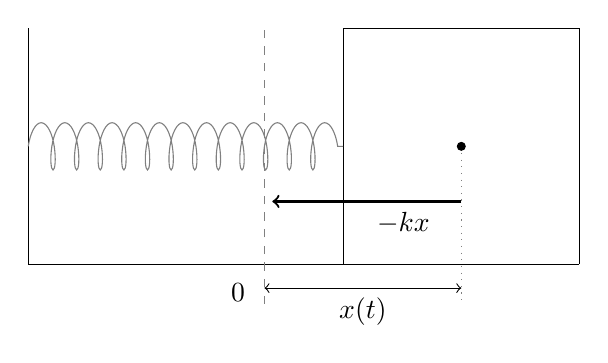
\begin{tikzpicture}
\draw[-] (0,0) -- (7,0);
\draw[-] (0,0) -- (0,3);

\draw[-] (4,0) -- (4,3) -- (7,3) -- (7,0);

\draw[gray,dashed] (3,-0.5) -- (3,3);
\draw[gray,dotted] (5.5,1.5) -- (5.5,-0.5);
\draw[thick,->] (5.5,0.8) -- node[below right, fill=white] {$-kx$} (3.1,0.8);
\node[label=below left:{$0$}] at (3,0) {};

\draw[gray,decoration={aspect=0.3, segment length=3mm, amplitude=3mm,coil},decorate] (0,1.5) -- (4,1.5);

\draw[<->] (3,-0.3) -- node[below] {$x(t)$} (5.5,-0.3);
\node[draw, fill=black, circle, inner sep=1pt] at (5.5,1.5) {};
\end{tikzpicture}
\caption{Sistema masa-resorte, con la fuerza del muelle $-kx$.}
\label{imgMasaResorte1}
\end{figure}

Según la ley de Hooke, la fuerza será

\[ F = -kx \]

donde $k$ es una constante que depende del muelle. Por la segunda ley de newton, tenemos que la fuerza es el producto de la masa y la aceleración,, por tanto, la ecuación que describe el movimiento es 

\[ mx'' = -kx \]

Podemos transformarla a un problema en derivadas ordinarias

$$\left\lbrace \begin{array}{l}
x'' + \frac{k}{m}x = 0\\
x(0) = x_0\\
x'(0) = v_0
\end{array}\right. $$

para el que necesitaremos posición y velocidad iniciales. 

El polinomio característico es

\[ λ^2 + \frac{k}{m} = 0 \]

cuyas raíces son 

\[ λ=\pm \i\sqrt{\frac{k}{m}} \]

Las soluciones complejas son, por lo tanto,

\begin{gather*}
z_1 = e^{\i t\sqrt{\frac{k}{m}}} = \cos \sqrt{\frac{k}{m}} t + \i \sin \sqrt{\frac{k}{m}} t \\
z_1 = e^{-\i t\sqrt{\frac{k}{m}}} = \cos \sqrt{\frac{k}{m}} t - \i \sin \sqrt{\frac{k}{m}} t 
\end{gather*}

Combinándolas de forma lineal, obtenemos dos soluciones reales:

\begin{gather*}
x_1(t) = \Re (z_1) = \cos \sqrt{\frac{k}{m}} t \\
x_2(t) = \Im (z_1) = \sin \sqrt{\frac{k}{m}} t
\end{gather*}

Aunque se ve a simple vista que esas dos soluciones son independientes (el coseno y el seno del mismo ángulo), deberíamos calcular el wronskiano para comprobar que son realmente independientes.

La solución general nos queda

\begin{equation}\label{eqMasaResorte} x(t) = A\cos \sqrt{\frac{k}{m}} t + B \sin \sqrt{\frac{k}{m}} 
\end{equation}

Las constantes $A$ y $B$ se tendrán que obtener una vez dados los valores iniciales. Si suponemos $x(0) = x_0$, $x'(0) = v_0$, tenemos que

\begin{gather*}
x_0 = x(0) = A \\
x'(t) = -x_0 \sqrt{\frac{k}{m}} \sin \sqrt{\frac{k}{m}} t + B \sqrt{\frac{k}{m}}\cos\sqrt{\frac{k}{m}} t \\
v_0 = x'(0) = B \sqrt{\frac{k}{m}} \\
B = \frac{v_0}{\sqrt{\frac{k}{m}}}
\end{gather*}

Si bien esta solución es correcta, los físicos suelen reescribirla de una forma distinta utilizando coordenadas polares para el punto $(A,B)$:

\begin{align*}
A &= R\cos φ \\
B &= R\sin φ 
\end{align*}

Sustituyendo en \eqref{eqMasaResorte}

\[ x(t) = R\left(\cos \sqrt{\frac{k}{m}} t\cos φ + \sin \sqrt{\frac{k}{m}} t \sin φ \right) = R\cos\left(\sqrt{\frac{k}{m}}t - Φ\right) \]

donde $Φ = \arctan \frac{B}{A}$ es el desfase, que actúa de velocidad inicial del sistema.

\paragraph{Sistema masa-resorte con rozamiento}

Replanteemos el problema anterior con rozamiento.
\begin{figure}
\centering
\begin{tikzpicture}
\draw[-] (0,0) -- (7,0);
\draw[-] (0,0) -- (0,3);

\draw[-] (4,0) -- (4,3) -- (7,3) -- (7,0);

\draw[gray,dashed] (3,-0.5) -- (3,3);
\draw[gray,dotted] (5.5,1.5) -- (5.5,-0.5);
\draw[thick,->] (5.5,2) -- node[above right, fill=white] {$-εx'$} (2.7,2);
\draw[thick,->] (5.5,0.8) -- node[below right, fill=white] {$-kx$} (3.1,0.8);
\node[label=below left:{$0$}] at (3,0) {};

\draw[gray,decoration={aspect=0.3, segment length=3mm, amplitude=3mm,coil},decorate] (0,1.5) -- (4,1.5);

\draw[<->] (3,-0.3) -- node[below] {$x(t)$} (5.5,-0.3);
\node[draw, fill=black, circle, inner sep=1pt] at (5.5,1.5) {};
\end{tikzpicture}
\caption{Sistema masa-resorte con rozamiento (fuerza $-εx'$).}
\end{figure}

La ecuación cambia al añadir el rozamiento:

\begin{gather} mx'' = -kx - εx' \nonumber \\
x'' + \frac{ε}{m}x' + \frac{k}{m}x = 0
\end{gather}

Resolvemos el polinomio característico \[ λ^2 + \frac{ε}{m}λ + \frac{k}{m} = 0 \] y nos queda

\[ λ = \frac{-ε}{2m} \pm \sqrt{\left(\frac{ε}{2m}\right)^2 - \frac{k}{m}} \].

Tenemos que plantear tres casos basados en el valor de $Δ =\left(\frac{ε}{2m}\right)^2 - \frac{k}{m}$: si es mayor, igual o menor que cero.

\subparagraph{Primer caso: $Δ > 0$ (rozamiento alto)}

Tenemos 

\begin{gather*}
λ_+ = \frac{-ε}{2m} + \sqrt{\left(\frac{ε}{2m}\right)^2 - \frac{k}{m}} \\
λ_- = \frac{-ε}{2m} - \sqrt{\left(\frac{ε}{2m}\right)^2 - \frac{k}{m}} 
\end{gather*}

De sus expresiones vemos que tanto $λ_+$ como $λ_-$ son negativos, puesto que la raíz siempre será menor que $\frac{\epsilon}{2m}$. La solución general del problema es 

\[ x(t) = Ae^{λ_+t} + Be^{λ_-t} \]

Despejando de los valores iniciales $x(0) = x_0$, $x'(0) = v_0$ y realizando ciertas operaciones,

\[ x(t) = \frac{1}{λ_+ - λ_-}\left((v_0-λ_-x_0)e^{λ_+t} - (v_0-λ_+x_0)e^{λ_-t}\right) \]

De esa ecuación vemos que, cuando $t\to ∞$, $x(t) \to 0$. Es decir, el objeto tiende a pararse.

También querríamos ver cuántas veces pasamos por la posición de equilibrio. Tenemos que resolver la ecuación

\[ e^{(λ_+ - λ_-)t} = \frac{v_0-λ_+x_0}{v_0-λ_-x_0} \]

que no tiene solución. Por lo tanto, el objeto no llega nunca a la posición de equilibrio.

\subparagraph{Segundo caso: $Δ=0$}

En este caso, tenemos $λ=\frac{-ε}{2m}$ que es una raíz doble. Por el método de variación de las constantes, nuestras dos soluciones son

\[ x_1(t) = e^{\frac{-ε}{2m}t};\quad x_2(t) = te^{\frac{-ε}{2m}t} \]

y la solución general se expresa como 

\[ x(t) = A e^{\frac{-ε}{2m}t} + B t e^{\frac{-ε}{2m}t} = e^{\frac{-ε}{2m}t} \left(A + Bt\right) \]

Al igual que en el anterior caso, $x(t) \convs[][t][∞] 0$, pero aquí sí que podemos tener soluciones para $x(t) = 0$.

\subparagraph{Tercer caso: $Δ < 0$ (sin rozamiento)}

Aquí tendremos raíces complejas, es decir:

\[ λ_+ = \frac{-ε}{2m} + \i \sqrt{\frac{k}{m} - \left(\frac{ε}{2m}\right)^2} \]

y su conjugada. De esta forma, las dos soluciones reales serán

\begin{gather*}
x_1(t) = e^{\frac{-ε}{2m}t} \cos t\sqrt{\frac{k}{m} - \left(\frac{ε}{2m}\right)^2} \\
x_1(t) = e^{\frac{-ε}{2m}t} \sin t\sqrt{\frac{k}{m} - \left(\frac{ε}{2m}\right)^2} \\
\end{gather*}

Podemos extraer la solución general y hacer el cambio del anterior apartado, pasando a polares $(A,B) \sim (R\cos φ, R\sin φ)$s, de tal forma que nos queda la solución general

\[ x(t) = R e^{-\frac{ε}{2m}t} \cos \left(t\sqrt{\frac{k}{m} - \left(\frac{ε}{2m}\right)^2} - Φ\right) \]

Es decir, hay un decaimiento exponencial de la amplitud. La gráfica de la función sería la de la \textbf{Figura \ref{fig:imgMasaResorteSeno}}

\img{img/MasaResorteSeno.png}{$x(t)$ para un sistema masa-resorte}{imgMasaResorteSeno}{0.8}

\paragraph{Péndulo simple}

Consideramos un péndulo simple sin rozamiento.

\begin{figure}[hbtp]
\centering
\begin{tikzpicture}
\draw[-] (-2,0) -- (2,0);
\draw[-] (0,1) -- (0,-4);

\draw[-] (0,0) -- (1,-2);
\draw[->] (1,-2) -- node[right] {$mg$} (1,-3.5);
\node[draw, fill=white, circle, inner sep=4pt] at (1,-2) {};
\end{tikzpicture}
\caption{El péndulo}
\end{figure}

Tenemos las ecuaciones de posición

\[ σ(t) = (L\sin θ(t), - L \cos θ(t))\]

de velocidad

\[ σ'(t) = (Lθ'(t)\cos θ(t), Lθ'(t)\sin θ(t))\]

y aceleración

\begin{align*}
 σ''(t) = (&-L(θ'(t))^2\sin(t) + Lθ''(t)\cos(t), \\
 & L(θ'(t))^2\cos θ(t) + Lθ''(t)\sin θ(t)) 
 \end{align*}.
 
Por la segunda ley de Newton, tenemos que la fuerza ejercida es igual al producto de la masa y la aceleración. Si dividimos la cuerda en su componente tangencial y perpendicular tenemos:

\[ mg( -\cosθ, -\sin θ)\sin θ  = m σ''(t) \]

y por lo tanto nos quedan las dos ecuaciones
\[ 
\left\{\begin{matrix}
 -g\sin θ \cos^2 θ = -L θ'^2 \cos θ \sin θ+ Lθ''\cos^2θ  \\
 -g\sin θ \sin^2 θ = -L θ'^2 \sin θ \cos θ  + Lθ''\sin^2θ  
 \end{matrix}\right\} \]
 
 La ecuación final es \[ -g\sin θ = L θ'' \] o, transformada 
 
 \[ θ'' + \frac{g}{L} \sin θ = 0 \]

Por Taylor, podemos aproximar $\sin θ \sim θ$ cuando θ es pequeña, de tal forma que nos reducimos al caso de un sistema masa-resorte.

\subsection{Problemas lineales no homogéneos con coeficientes constantes}

¿Qué ocurre cuando consideramos sistemas con fuerzas externas? Un ejemplo sería la siguiente ecuación en orden dos:

\begin{equation}
\label{eqEcOrden2} x'' + ax' + bx = f(t)
\end{equation}

en la que $f(t)$ representa esa fuerza externa. Tal y como habíamos visto en anteriores secciones, la solución general $X_G$ se escribía como una solución particular $X_P$ más todas las asociadas al homogéneo $X_H$. En esta situación el problema es encontrar la solución particular, para lo cual teníamos varios métodos.

\subsubsection{Método de variación de constantes}
\label{secMetodoVarConst}
\index{Variación!de constantes} 

Siguiendo con el ejemplo en orden 2, tenemos 

\[ x_H (t) = c_1x_1(t) + c_2x_2(t) \]
y buscamos una solución en la que
$$
\left\lbrace
\begin{array}{l}
c_1 = c_1(t)\\
c_2 = c_2(t)
\end{array}
\right. 
$$
Por tanto buscamos $X_P$ tal que
\[ x_P(t) = c_1(t)x_1(t) + c_2(t)x_2(t) \] Para ello derivamos:
\begin{align*}
x_P'&= c_1'x_1 + c_1x_1' + c_2'x_2 + c_2x_2' = \\
	&= c_1'x_1 + c_1 \\
x_P'' 	&= c_1''x_1+c_1'x_1' + c_2''x_2+c_2'x_2' + \\ 
		&\quad+ c_1'x_1'+c_1x_1'' + c_2'x_2' + c_2x_2'' = \\
		&= x_1''x_1 + c_2''x_2+2c_1'x_1'+2c_2'x_2' + c_1x_1'' +c_2x_2'' 
\end{align*}

Sustituyendo en \eqref{eqEcOrden2}:

\begin{align*}
f(t) &= x_P'' + ax_P' + bx_P = &  \\
	&= c_1''x_1 + c_2''x_2 + 2c_1'x_1' + 2c_2'x_2'  + c_1x_1''  + c_2x_2'' \\
	& + ac_1' x_1 + ac_2'x_2  + ac_1x_1'  + ac_2x_2' \\
	&  + bc_1x_1  + bc_2x_2 
\end{align*}

Tras la sustitución tenemos una expresión bastante compleja. Sin embargo, recordamos que no buscamos todas las soluciones de la ecuación, sino que basta con encontrar sólo una. Por ello, planteamos ciertas condiciones para resolver la expresión hallada:

$$ \left\lbrace \begin{array}{l}
c_1'x_1 + c_2'x_2 = 0 \\  
c_1'x_1' + c_2'x_2' = f
\end{array} \right. $$
Que nos lleva al sistema

\[ \underbrace{\begin{pmatrix}
x_1 & x_2 \\
x_1' & x_2' 
\end{pmatrix}}_A\begin{pmatrix}
c_1' \\ c_2'
\end{pmatrix} = \begin{pmatrix}
0 \\ f(t)
\end{pmatrix} \] 
Se puede obserbar que el sistema tiene solución, ya que al ser $x_1,\ x_2$ soluciones independientes, el Wronskiano (en este caso, el determinante de $A$ es distinto de $0$).

En un caso general de orden $n$, el sistema a plantear tendrá la siguiente forma

\[ \begin{pmatrix}
x_1 & \cdots & x_n \\
x_1' & \cdots & x_n \\
\vdots & \ddots & \vdots \\
x_1^{n)} & \cdots & x_n^{n)}
\end{pmatrix} \begin{pmatrix} c_1' \\ c_2' \\ \vdots \\ c_n' \end{pmatrix} 
= 
\begin{pmatrix}
0 \\ \vdots \\ 0 \\ f(t)
\end{pmatrix} \]
Veamos un ejemplo.

\begin{example}
$x'' + x = e^t$

Buscamos $x_P(t) = c_1(t) x_1 + c_2(t) x_2$, donde

\[ \underbrace{\begin{pmatrix}
x_1 & x_2 \\
x_1' & x_2' 
\end{pmatrix}}_A\begin{pmatrix}
c_1' \\ c_2'
\end{pmatrix} = \begin{pmatrix}
0 \\ e^t
\end{pmatrix} \] 

Podemos elegir $x_1$ y $x_2$ como el seno y el coseno de $t$:

\[ \underbrace{\begin{pmatrix}
\cos t & \sin t \\
- \sin t & \cos t 
\end{pmatrix}}_A\begin{pmatrix}
c_1' \\ c_2'
\end{pmatrix} = \begin{pmatrix}
0 \\ e^t
\end{pmatrix} \] 
Resolviendo el sistema nos queda que 

\[ c_2' = e^t \cos t \]

Realizando bastantes operacioens podemos obtener una solución particular, sin embargo, podemos darnos cuenta de que una de las soluciones particulares es

\[ x_p(t) = \frac{e^t}{2} \]

¿Qué tiene de especial este problema? La exponencial en $f(t)$. Lo que nos lleva a estudiar otro método, el de coeficientes indeterminados.
\end{example}





\newpage
\mbox{}
\thispagestyle{empty}
\newpage
\appendix
\section{Algunos problemas clásicos}
A continuación vamos a abordar un el problema de la catenaria y lo solucionaremos aplicando alguna de las técnicas de integración estudiadas.

\img{img/catenaria.png}{Curva catenaria}{catenaria}{0.8}
\begin{example}[(Problema de la catenaria)]
El problema de la catenaria trata de encontrar una expresión para la curva que describe una cadena que cuelga de dos puntos (ver \textbf{Figura \ref{fig:catenaria}}).
Para encontrar esta expresión, vamos a estudiar sólo un trozo de la cadena, que en la figura se muestra de color negro oscuro.

Para que la sección de cadena esté en equilibrio, tiene que haber dos fuerzas que la sujeten por los puntos $A$ y $B$. 

\begin{itemize}
\item En el punto $A$ tenemos el vector $T$, que tiene que tener la dirección de la tangente a la curva. Denotaremos como $T_x$ a la componente horizontal y como $T_y$ a la componente vertical.

La componente $T_y$ tiene que contrarrestar al peso del segmento de cadena, que viene dado por el producto entre su densidad y su longitud. La densidad la denotaremos por $\rho$ y la longitud es $\int_0^x \norm{\sigma^\prime(s)}ds$, donde $x$ es la primera coordenada de $A$ y $\sigma$ es la parametrización de la curva $\sigma = (x, y(x))$. Por tanto el peso será $\int_0^x \sqrt{1+(y^\prime(ds))^2}ds$.

\item En el punto $B$ el segmento ha de ser sujetado por una fuerza que contrarreste a $T_x$.
\end{itemize}

Tenemos entonces los siguientes datos:
\begin{equation*}
  \left\lbrace
  \begin{array}{l}
     T_x = Tcos(\alpha)=T_0 \text{(Tensión)} \\
     T_y = Tsin(\alpha) = \rho\int_0^x \sqrt{1+(y^\prime(ds))^2}ds \\
     tan(\alpha) = y^\prime(x)\\
  \end{array}
  \right.
\end{equation*}
Dividiendo la segunda expresión por la primera: 
$$\frac{sin(\alpha)}{cos(\alpha)} = \frac{\rho}{T_0}\int_0^x \sqrt{1+(y^\prime(ds))^2}ds$$
Utilizando la tercera:
$$y^\prime(x) = \frac{\rho}{T_0}\int_0^x \sqrt{1+(y^\prime(ds))^2}ds$$
Derivando para que desaparezca la integral:
$$y^{\prime\prime}(x) = \frac{\rho}{T_0}\sqrt{1+(y^\prime(x))^2}$$
Tenemos una ecuación de segundo orden, que sabemos convertir en un sistema de dos ecuaciones de primer orden:
\begin{equation*}
  \left\lbrace
  \begin{array}{l}
     y^\prime = p \\
     p^\prime(x) = \frac{\rho}{T_0}\sqrt{1+p^2(x)} \\
  \end{array}
  \right.
\end{equation*}
con los datos $p(0) = 0$ y $y(L) = H$ donde $A = (L,H)$.
Notamos ahora que estamos ante una EDO separable:
$$\frac{p^\prime(x)}{\sqrt{1+p^2(x)}} = \frac{\rho}{T_0}$$
Integrando ambos términos:
$$\int_0^x \frac{p^\prime(s)}{\sqrt{1+p^2(s)}}ds = \frac{\rho}{T_0}\int_0^x ds = \frac{\rho}{T_0}x$$
Realizando el cambio de variables $
  \left\lbrace
  \begin{array}{l}
     p(s) = u \\
     p^\prime(s)ds = du \\
  \end{array}
  \right.
$

obtenemos $$\int_0^{p(x)} \frac{du}{\sqrt{1+u^2}} = \frac{\rho}{T_0} x $$
Para resolver esta integral se puede usar que $cosh^2(z) = 1+ sinh^2(z)$ y realizar un cambio de variables. Tenemos entonces que $$ln(\sqrt{1+p(x)} + p(x)) = \frac{\rho}{T_0} x $$
Tomando exponenciales y despejando $p$ llegamos a que
$$y^\prime = p = \frac{e^{\frac{\rho}{T_0} x }-e^{\frac{-\rho}{T_0} x }}{2} = sinh(\frac{\rho}{T_0} x )$$
Integrando de nuevo llegamos a la solución:
$$y = \frac{T_0}{\rho}cosh(\frac{\rho}{T_0} x ) + C$$
donde podemos obtener la constante utilizando los datos ya proporcionados.
\end{example}

\img{img/puente.png}{Puente Colgante}{puente}{0.8}

\begin{example}
En el ejemplo anterior, hemos visto el problema de la caternaria. Cambiemos algunas hipótesis iniciales:
\begin{itemize}
\item Supongamos que ahora tenemos un puente colgante y queremos averiguar una expresión para la curva que describe la cadena que sujeta la calzada.
\item La calzada se sujeta con cuerdas cuyo peso es despreciable.
\end{itemize}
Para la resolución de este problema, el método a seguir es el mismo que en el ejemplo anterior. Sin embargo, ahora la componente $T_y$ no tiene que sujetar el peso de la cuerda, sino el peso del puente, que es en este caso el producto de su densidad $C$ y su longitud $x$. (Ver \textbf{Figura \ref{fig:puente}}).

Tenemos entonces
\begin{equation*}
  \left\lbrace
  \begin{array}{l}
     T_x = Tcos(\alpha)=T_0 \text{(Tensión)} \\
     T_y = Tsin(\alpha) = Cx \\
     tan(\alpha) = y^\prime(x)\\
  \end{array}
  \right.
\end{equation*}

De donde obtenemos que $y^\prime = \frac{C}{T_0}x$
Por lo que la solución es $$y = \frac{C}{2T_0}x^2 + D$$
\end{example}

\begin{example}
Supongamos que se tiene una cortina colgada de dos extremos. En este caso, al contrario que en el ejemplo anterior, el peso se distribuye por todo el área encerrada bajo la curva de la cortina. Por tanto, la ecuación diferencial obtenida será $$y^\prime = \frac{c}{T_0}\int_0^x y(s)ds$$ de donde obtenemos $$y^{\prime\prime} = \frac{c}{T_0}y$$

Basta con tomar $y^\prime = p$ y $y^{\prime\prime} = p\partialder{y}{p}$

Obtenemos entonces que $$p\partialder{y}{p} = \frac{c}{T_0}y$$ 
Integrando ambos términos tenemos $$\frac{1}{2}p^2(y) = \frac{c}{2T_0}y^2+D$$
$$y^\prime = p = \sqrt{\frac{c}{T_0}y^2+D}$$
obteniendo así una EDO de primer orden.
\end{example}

\img{img/brac.png}{Curva braquistocrona}{brac}{0.7}

\begin{example}[(Braquistocrona I)]
El objetivo de este problema es encontrar la expresión de la curva en la que el tiempo de descenso es mínimo al soltar un cuerpo que se deslice por ella (Ver \textbf{Figura \ref{fig:brac}}).

Vamos a parametrizar la curva en función del tiempo, de modo que obtenemos
$$\sigma(t) = (x(t),y(x(t)))$$
$$\sigma^\prime(t) = (x^\prime(t), \partialder{x}{y}(x(t))x^\prime(t))$$
$$\norm{\sigma^\prime(t)} = \abs{x^\prime(t)}\sqrt{1+(\partialder{x}{y}(x(t)))^2}$$


Aplicando unos pocos conocimientos físicos notamos que la energía cinética ha de ser igual a la potencial, pues despreciamos el rozamiento. Tenemos entonces
$$\frac{1}{2}mv^2 = mg(-y) \implies v = \sqrt{-2gy}$$

Igualando estas dos expresiones para la velocidad llegamos a la expresión
$$\sqrt{\frac{1+(\partialder{x}{y}x(t))^2}{-2gy(x(t))}}x^\prime(t) = 1$$

Ahora integramos ambos términos entre $0$ y $T$, siendo $T$ el tiempo de llegada
$$\int_0^{T}\sqrt{\frac{1+(\partialder{x(t)}{y}x(t))^2}{-2gy(x)}}x^\prime(t) = T$$
y realizamos el cambio de variable $x(t) = x$. Tenemos entonces que los límites de integración son ahora $0$ y $x_B$.
$$\int_0^{x_B}\sqrt{\frac{1+(\partialder{x}{y}x)^2}{-2gy(x)}}dx = T$$

Como resultado de lo anterior, tenemos una función que indica el tiempo de llegada al punto de destino.
Como hemos dicho al inicio, el objetivo es minimizar ese tiempo. Por tanto, buscamos el mínimo de la función
$$T(y) = \int_0^{x_B}\sqrt{\frac{1+(\partialder{x}{y}x)^2}{-2gy(x)}}dx$$
$$T(y) = \int_0^{x_B} F(y, \partialder{x}{y})dx$$
$$T(y) = \int_0^{x_B} F(y, p)dx$$

Esta función toma una función y devuelve un número, por lo que es dificil de manejar. Si definimos
$$T(y+\delta\Phi) = g(\delta)$$
siendo $y$ la solución del problema y $\Phi$ una función que pertenezca al conjunto 
$$A = \set{f:[0,x_B] \to \R \st f\in C^1, f(0) = 0, f(x_B) = 0}$$
tenemos que $g(0)$ es un mínimo de $T(y)$.

Tenemos entonces $$g(\delta) = \int_0^{x_B} F(y+\delta\Phi, \derivative{x}(y+\delta\Phi)dx$$
$$g(\delta) = \int_0^{x_B} F(y+\delta\Phi, \partialder{x}{y} + \delta\partialder{x}{\Phi})dx$$

Como $0$ es un punto crítico de $g$, tenemos que $g^\prime(0) = 0$
$$g^\prime(0) = \derivative{\delta}(0) = \int_0^{x_B} F(y+\delta\Phi, \partialder{x}{y} + \delta\partialder{x}{\Phi})dx = 0$$

$$g^\prime(0) = \int_0^{x_B} \partialder{y}{F}\Phi + \partialder{p}{F}\partialder{x}{\Phi}dx = 0$$

Integrando el segundo término de la integral por partes, llegamos a que

$$g^\prime(0) = \int_0^{x_B} (\partialder{y}{F}-\derivative{x}\partialder{p}{F})\Phi dx = 0 \forall \Phi\in A$$

Tenemos entonces la EDO
$$\partialder{y}{F}-\derivative{x}\partialder{p}{F} = 0$$

Multiplicando a ambos lados por $\partialder{x}{y}$
$$\derivative{x}(F-\partialder{x}{y}\partialder{p}{F} = 0$$
$$F-\partialder{x}{y}\partialder{p}{F} = cte$$

Retomando la función $F$ definida anteriormente tenemos y realizando los calculos necesarios para sustituir en la EDO tenemos
$$\frac{\sqrt{1+(y^\prime)^2}}{\sqrt{2y}\sqrt{-y}}-y^\prime\frac{1}{\sqrt{2y}}\frac{1}{\sqrt{-y}}\frac{y^\prime}{\sqrt{1+(y^\prime)^2}}=C$$

Tras varias operaciones de simplificación obtenemos
\begin{equation*}
  \left\lbrace
  \begin{array}{l}
     y^\prime=-\sqrt{\frac{-1}{2gc^2y}-1}\\
	 y(x_B)=y_B\\
  \end{array}
  \right.
\end{equation*}

Tras resolver este problema, que se deja como ejercicio para el lector, se obtiene una curva cicloide.
\vspace{5mm}
\textit{Indicación: Denotar} $$k = \frac{1}{-2gc^2}$$ \textit{y realizar, a la hora de integrar, el cambio de variables} $$1+tan^2(x(=\frac{1}{cos^2(x)}$$
\end{example}

\img{img/brac2.png}{}{brac2}{0.7}

\begin{example}[(Braquistocrona II)]
Otra forma de resolver el problema de la braquistocrona es aplicando resultados fisicos de la óptica.
Según la ley de Snell, cuando la luz pasa de un medio a otro, se cumple que
$$\frac{sin(\alpha_1)}{v_1} = \frac{sin(\alpha_2)}{v_2}$$

Si dividimos el espacio en bandas horizontales de longitud $h$ en las que en cada banda está la tangente a la curva (Ver \textbf{Figura \ref{fig:brac2}}), tenemos la relación
$$\frac{sin(\alpha_1)}{v_1} = \frac{sin(\alpha_2)}{v_2} = \hdots$$

Cuando $h\to 0$ tenemos que $\frac{sin(\alpha)}{v} = cte$ por lo que obtenemos
$$\frac{sin(\alpha)}{\sqrt{-2gy}}=C$$

Sabiendo que $tan(\alpha+\frac{\pi}{2}) = y^\prime$, con la ecuación anterior obtenemos una EDO que satisface la curva.
\end{example}

\printindex
\end{document}
